\section{A brief history of geometry}

    Differential geometry is the language in which general relativity is written, and like every language it was not designed in advance for the use we are about to make of it, it grew slowly, over more than four thousand years, out of problems that had nothing to do with gravity. Before we start defining manifolds and tangent spaces it is worth spending a few pages on where these ideas came from, because \textbf{almost every object we are going to construct in this chapter was invented by someone who had no idea that physics would one day need it}, and knowing that history makes the definitions feel far less arbitrary than they otherwise might.

    \subsection{Geometry as the measurement of the earth}

        The word itself confesses the origin: \textit{geometry} comes from the Greek $\gamma\epsilon\omega\mu\epsilon\tau\rho\acute{\iota}\alpha$, built from $\gamma\tilde{\eta}$ (earth) and $\mu\acute{\epsilon}\tau\rho o\nu$ (measure), so that the name of the discipline literally means \textit{earth measurement}. Herodotus, writing in the fifth century B.C., tells us in the second book of his \textit{Histories} that geometry was invented in Egypt for an entirely practical reason: the Nile flooded every year, washing away the boundary markers of the fields along its banks, and since the pharaoh taxed each landholder in proportion to the area he held, somebody had to go out after every flood and measure the land again \citep{herodotus_histories}. The men who did this were the \textit{harpedonaptai}, the rope stretchers, and they worked with knotted cords that let them lay out right angles in the field by the simple trick of forming a triangle with sides in the ratio three, four and five.

        The Babylonians were, if anything, further ahead. The clay tablet catalogued as Plimpton 322, dated to roughly 1800 B.C., lists what we would now call Pythagorean triples, several centuries before Pythagoras was born, and the Egyptian Rhind papyrus of about 1650 B.C. contains worked recipes for the areas of triangles and circles together with a remarkably good approximation to $\pi$. What none of these documents contain, however, is a single proof. \textbf{Geometry began as an empirical and practical science, a catalogue of recipes that worked}, with no axioms, no deductive structure and no claim whatsoever to necessary truth, and it would take the Greeks to change that.

    \subsection{Euclid and the tyranny of the fifth postulate}

        Around 300 B.C., in the Alexandria we already visited in chapter 1, Euclid gathered essentially everything the Greek world knew about geometry into the thirteen books of the \textit{Elements}, and in doing so he invented something far more valuable than any individual theorem: the axiomatic method itself \citep{euclid_elements}. Euclid begins with definitions, five common notions and five postulates, and from that small seed he deduces four hundred and sixty five propositions, each one following from what came before with a logical necessity that had never been demanded of mathematics before. For the next two thousand years the \textit{Elements} was not merely a textbook of geometry, it was the model of what secure knowledge was supposed to look like, and Newton's \textit{Principia}, as we saw, is written deliberately in its style.

        There was, however, a splinter in this perfect structure, and everybody could feel it. Euclid's first four postulates are short, obvious and almost embarrassingly modest: a straight line can be drawn between any two points, a finite line can be extended indefinitely, a circle can be drawn with any centre and radius, and all right angles are equal. The fifth is nothing like them. In Euclid's own formulation it states that if a straight line falling on two straight lines makes the interior angles on the same side less than two right angles, then those two lines, extended far enough, will meet on that side, a statement so long, so conditional and so manifestly \textit{unobvious} that it reads like a theorem somebody failed to prove and quietly promoted. Euclid himself seems to have been uneasy about it, because he avoids using it for as long as he possibly can, delaying its first appearance until Proposition 29. By the fifth century A.D. Proclus was already arguing openly that the fifth postulate ought to be struck from the list of assumptions and derived from the other four, and \textbf{the attempt to do exactly that became the longest running unsolved problem in the history of mathematics}.

    \subsection{The long assault on the parallel postulate}

        The assault was genuinely international and it lasted the better part of two millennia. Working in the same Islamic mathematical tradition we met in chapter 1, Ibn al-Haytham attacked the problem in the eleventh century using a quadrilateral with three right angles, the Persian poet and mathematician Omar Khayyam (1048 to 1131) refined the approach considerably, and Nasir al-Din al-Tusi (1201 to 1274), whose Tusi couple we have already encountered, produced a treatment careful enough that it eventually reached Europe and was discussed by John Wallis at Oxford in the seventeenth century \citep{kline1972}.

        The decisive attempt, and the most poignant, came from the Italian Jesuit Girolamo Saccheri, who published in 1733, the year of his death, a book with the triumphant title \textit{Euclides ab omni naevo vindicatus}, Euclid freed of every flaw \citep{saccheri1733}. Saccheri's strategy was \textit{reductio ad absurdum}: he assumed the fifth postulate to be false, and then set out to derive a contradiction. He worked with enormous patience and skill, deducing theorem after theorem from the negated postulate, and what he found was that the consequences were strange (triangles whose angles sum to less than two right angles, no similar figures of different sizes, an absolute unit of length built into space itself) but that they were also, maddeningly, perfectly consistent with one another. No contradiction ever came. At the end, unable to produce the absurdity his whole book was built to produce, Saccheri simply declared that the resulting propositions were \textit{repugnant to the nature of the straight line} and announced the job done. \textbf{Saccheri had derived, theorem by theorem, a substantial part of hyperbolic geometry, and then refused to believe what he was looking at.} Johann Heinrich Lambert went further still a few decades later, and came even closer to accepting the conclusion, but he too stopped short of publishing it as a discovery rather than a failure.

    \subsection{The birth of non-Euclidean geometry}

        The break, when it finally came, came three times at once. Gauss had convinced himself privately, somewhere in the 1810s and 1820s, that a perfectly consistent geometry could be built in which the parallel postulate fails, and he never published a word of it. His reason, given in a letter to Bessel of January 1829, is one of the more human documents in the history of mathematics: he feared, he wrote, \textit{das Geschrei der Böotier}, the clamour of the Boeotians, the Boeotians being the Greek byword for provincial stupidity, and he had no appetite for the controversy that publication would bring down on him \citep{kline1972}.

        Nikolai Ivanovich Lobachevsky, working at the University of Kazan far out on the Russian frontier, had no such caution and published his account of what he called imaginary geometry in 1829 \citep{lobachevsky1829}. Independently, in Hungary, the young army officer János Bolyai reached the same conclusions and published them in 1832 as a twenty four page appendix to a mathematics textbook written by his father Farkas \citep{bolyai1832}. Bolyai had written to his father about the discovery nine years earlier, in November 1823, with a line that every student of geometry should know: \textit{out of nothing I have created a strange new universe}. Farkas, who had himself wasted years on the parallel postulate and who happened to be an old friend of Gauss, proudly forwarded the appendix to Göttingen for an opinion. Gauss's reply was, by any reasonable standard, a disaster: he explained that he could not praise the work, because to praise it would be to praise himself, since he had held the same views for thirty or thirty five years already. János Bolyai, twenty nine years old and convinced he had been robbed, never published mathematics again.

        Set aside the human wreckage and the mathematical content is this: \textbf{the parallel postulate is independent of the other four, so Euclidean geometry is not the only possible geometry, it is merely one of several}, and therefore the question of which geometry describes the physical space we actually inhabit stops being a matter of pure logic and becomes an empirical question, to be settled by measurement. That single shift in status is what eventually made general relativity thinkable at all.

    \subsection{Gauss, Riemann and the turn inwards}

        The second decisive step was Gauss's, and we have already met it in chapter 1, though it is worth restating here from the mathematician's side rather than the physicist's. In the \textit{Disquisitiones generales circa superficies curvas} of 1827 Gauss proved his \textit{Theorema Egregium}, showing that the curvature of a surface can be computed entirely from measurements made within the surface itself \citep{gauss1828}. The consequence is philosophical as much as technical: a two dimensional creature confined to a curved surface, with no access whatsoever to a third dimension, could still determine that its world is curved, simply by measuring the angles of triangles or the circumferences of circles and comparing them with what flat geometry predicts. \textbf{Curvature stopped being something a space is seen to have from outside, and became something a space possesses in itself.}

        Bernhard Riemann's 1854 habilitation lecture, delivered before Gauss himself, then took this intrinsic point of view and released it from the restriction to two dimensional surfaces sitting in ordinary space \citep{riemann1873}. Riemann introduced what we would now call an $n$ dimensional manifold, a space that need only look like $\mathbb{R}^n$ in the neighbourhood of each of its points, and he showed how to put a \textit{metric} on such a space, a rule assigning a length to every infinitesimal displacement, from which curvature could then be computed at every point by pure calculation. Every single object in the remainder of this chapter, the manifold, the chart, the tangent space, the metric and ultimately the curvature tensor, descends directly from that one lecture, and Riemann's closing suggestion that the metric of physical space might be determined by the matter within it is the prophecy we discussed at length in chapter 1.

    \subsection{From absolute differential calculus to the modern theory}

        Riemann had the ideas but not yet a usable calculus, and supplying one occupied the next half century. Elwin Bruno Christoffel worked out in 1869 how the derivatives of the metric combine into the symbols that now bear his name and that we shall meet in chapter 3 \citep{christoffel1869}, and Gregorio Ricci-Curbastro, together with his student Tullio Levi-Civita, spent the 1880s and 1890s systematising the whole subject into what they published in 1900 under the name \textit{absolute differential calculus} \citep{ricci1900}. Their central concern was exactly the one that matters to a physicist: how to write equations whose form does not depend on the coordinate system used to express them, which is to say, how to do calculus with tensors. This is the paper, and this the machinery, that Marcel Grossmann put into Einstein's hands in 1912. Levi-Civita then added the missing geometrical idea in 1917, the notion of \textit{parallel transport}, which finally explained what it means to compare vectors at different points of a curved space \citep{levicivita1917}.

        Alongside this ran a second, more structural current. Felix Klein's Erlangen programme of 1872 proposed that a geometry is best understood not through its objects but through its symmetries, as the study of those properties left invariant by a group of transformations \citep{klein1872}, a point of view that runs straight into modern physics and that we shall use implicitly every time we demand that a physical law be invariant under Lorentz transformations. Élie Cartan rebuilt the subject again in the 1920s with his moving frames and his exterior calculus of differential forms, Hermann Weyl wrote the first genuinely geometrical textbook treatment of relativity in \textit{Raum, Zeit, Materie} in 1918 \citep{weyl1918}, and it was only in 1936 that Hassler Whitney finally proved the theorems that let us treat an abstract manifold as an object in its own right rather than as a surface embedded in some larger Euclidean space \citep{whitney1936}. That date is worth pausing on, because it is twenty one years \textit{after} the field equations were published: \textbf{Einstein built general relativity out of mathematics that was still being invented around him}, and the clean, coordinate free formulation that we now teach to students was largely assembled afterwards, in response to the theory rather than in preparation for it.

    \subsection{Why differential geometry is the language of relativity}

        It remains to say plainly why a physicist should care about any of this, and the answer is that every structural feature of general relativity is already a demand for differential geometry. The equivalence principle, which we shall state carefully in chapter 3, says that a freely falling observer detects no gravitational field in a sufficiently small neighbourhood of themselves, which is to say that \textit{space-time looks flat locally even when it is curved globally}, and this is precisely and exactly the defining property of a manifold, a space that is locally $\mathbb{R}^n$ without being globally anything of the sort. The principle of general covariance, that the laws of physics cannot depend on the coordinates chosen to write them down, forces us to work with objects defined independently of any chart, which is to say with tensors, and it is the reason we shall spend so much of this chapter on how components transform. Gauss's theorem that curvature is intrinsic is what allows us to speak of the curvature of space-time at all without embarrassing ourselves by having to ask what higher dimensional space it is supposedly curving into, since there is none and none is needed. Tidal forces, the one part of Newtonian gravity that genuinely cannot be transformed away by falling freely, turn out to be nothing other than the curvature tensor acting on a family of neighbouring geodesics, as we shall prove when we reach the equation of geodesic deviation. And the metric tensor, Riemann's rule for measuring infinitesimal distances, does double duty in relativity as both the ruler that measures space-time intervals and the gravitational potential itself, so that \textbf{in general relativity geometry and gravitation are not analogous to one another, they are the same thing described in two vocabularies}. What follows in this chapter is the construction of that vocabulary, from the ground up.

\section{Differentiable manifolds}

    This is one of the most attractive theories in physics and mathematics, because it allowed physicists to arrive at one of the most important theories of modern physics, general relativity, a geometrical theory of space and time bound together into a single entity called \textit{space-time}, with all the implications for our reality that this carries, since the theory allowed us to see beyond our planet, to dream of travelling beyond this earth and to describe genuinely strange systems, galaxies or universes. Here we are going to study briefly the foundations of differential geometry and of differentiable manifolds.

    If we wanted to make a completely rigorous study of differential geometry we should begin with set theory, then topology, then manifolds, and only then arrive at differentiable manifolds. We shall take a shorter road, but it is worth knowing which stations we are skipping.

    \subsection{A dictionary for the physicist}

        Before we start it is worth confronting a difficulty which has nothing to do with the mathematics itself and everything to do with the fact that mathematicians and physicists have spent a century describing the very same objects with different words. A student arriving here from a physics degree already knows most of these objects perfectly well and has been computing with them since the second year, so what makes the first encounter with differential geometry so uncomfortable is usually not that the content is new but that the names are. Because of that, and before writing down a single definition, we are going to lay out a small dictionary in table \ref{tab:Dictionary}, which the reader should feel entirely free to come back to as often as necessary, since almost everything appearing in it will only be properly defined in the pages that follow.

        \begin{table}[ht]
            \centering
            \small
            \begin{tabular}{p{0.25\textwidth} p{0.15\textwidth} p{0.46\textwidth}}
                \hline
                \textbf{Geometrical object} & \textbf{Components} & \textbf{What a physicist calls it, and where it appears}\\
                \hline
                Smooth function, $\binom{0}{0}$ & $f$ & Scalar field: a temperature, the Newtonian potential $\varphi$\\
                Tangent vector, $\binom{1}{0}$ & $X^{\mu}$ & Vector, or contravariant vector: the four velocity $u^{\mu}$\\
                Covector, $\binom{0}{1}$ & $\omega_{\mu}$ & Covariant vector, or one-form: the gradient $\partial_{\mu}f$, the four momentum $p_{\mu}$\\
                $\binom{1}{1}$ tensor & $A^{\mu}_{\;\nu}$ & A linear operator, in practice a matrix: the Kronecker delta $\delta^{\mu}_{\;\nu}$\\
                Symmetric $\binom{0}{2}$ tensor & $g_{\mu\nu}$ & The metric: it measures intervals and doubles as the gravitational potential\\
                Antisymmetric $\binom{0}{2}$ tensor & $F_{\mu\nu}$ & The Faraday tensor: the electric and magnetic fields packed into one object\\
                Symmetric $\binom{2}{0}$ tensor & $T^{\mu\nu}$ & The energy momentum tensor: the source term in Einstein's equations\\
                $\binom{1}{3}$ tensor & $R^{\rho}_{\;\sigma\mu\nu}$ & The Riemann tensor: the curvature, which is to say the tidal field\\
                \hline
            \end{tabular}
            \caption{A dictionary between the coordinate free language of differential geometry, the index notation of the working relativist, and the objects a physicist has already met somewhere else.}
            \label{tab:Dictionary}
        \end{table}

        The same translation problem happens with the vocabulary itself, so it is worth listing the most important pairs before we meet them one by one. When a mathematician says \textit{manifold} a physicist should hear \textit{the space, or the space-time, in which everything happens}; when the mathematician says \textit{chart} the physicist should hear \textit{coordinate system}, or more physically \textit{reference frame}; an \textit{atlas} is nothing more sinister than the complete collection of coordinate patches needed to cover everything without leaving holes; \textit{smooth} means differentiable as many times as we happen to need; the \textit{tangent space} $T_p(M)$ is the space of all the velocities a particle could possibly have as it goes through that event; and a \textit{diffeomorphism} is, for almost all of our purposes, a change of coordinates. \textbf{None of the geometry in this chapter is harder than the physics the reader already knows, it is simply written in a language built to survive without coordinates}, and that last property is exactly why general relativity cannot do without it. Readers who want the same material developed at greater length and with a physicist's priorities throughout will find it in \citet{schutz1980} and in \citet{nakahara2003}, while \citet{wald1984} is the standard place to look when we want the mathematician's version of a statement we have treated lightly here.

    \subsection{Manifolds, charts and atlases}

    \begin{myDef}
        An $n$-dimensional differentiable manifold is a set $M$ together with a collection of subsets $\mathcal{O}_{\alpha}$ such that:
    \end{myDef}

    \begin{enumerate}
        \item $\bigcup_{\alpha}\mathcal{O}_{\alpha} = M$. This means that the union of all the subsets covers the manifold $M$, so that every point of $M$ lies in at least one of them.

        \item For every $\alpha$ there exists a bijective map $\phi_{\alpha}$ onto an open subset $U_{\alpha} \subset \mathbb{R}^n$,

        \begin{equation}
            \begin{split}
                \phi_{\alpha}\;:\;\mathcal{O}_{\alpha} &\longrightarrow U_{\alpha} \subset \mathbb{R}^n\\
                p &\longmapsto \phi_{\alpha}(p) = \left(x_{\alpha}^1(p),\;...\;,x_{\alpha}^n(p)\right).
            \end{split}
        \end{equation}

        \item If $\mathcal{O}_{\alpha}$ and $\mathcal{O}_{\beta}$ intersect, so that $\mathcal{O}_{\alpha} \cap \mathcal{O}_{\beta} \neq \emptyset$, then the composition $\phi_{\beta} \circ \phi_{\alpha}^{-1}$ maps

        \begin{equation}
            \begin{split}
                \phi_{\beta} \circ \phi_{\alpha}^{-1}\;:\;\phi_{\alpha}\left( \mathcal{O}_{\alpha} \cap \mathcal{O}_{\beta} \right) \subset \mathbb{R}^n &\longrightarrow \phi_{\beta}\left( \mathcal{O}_{\alpha} \cap \mathcal{O}_{\beta} \right) \subset \mathbb{R}^n\\
                x &\longmapsto \left(\phi_{\beta} \circ \phi_{\alpha}^{-1}\right)(x),
            \end{split}
        \end{equation}

        and this map, which is a map between open subsets of $\mathbb{R}^n$ and therefore an ordinary object of multivariable calculus, must be smooth, that is, infinitely differentiable.

        \begin{figure}[h]
            \centering
            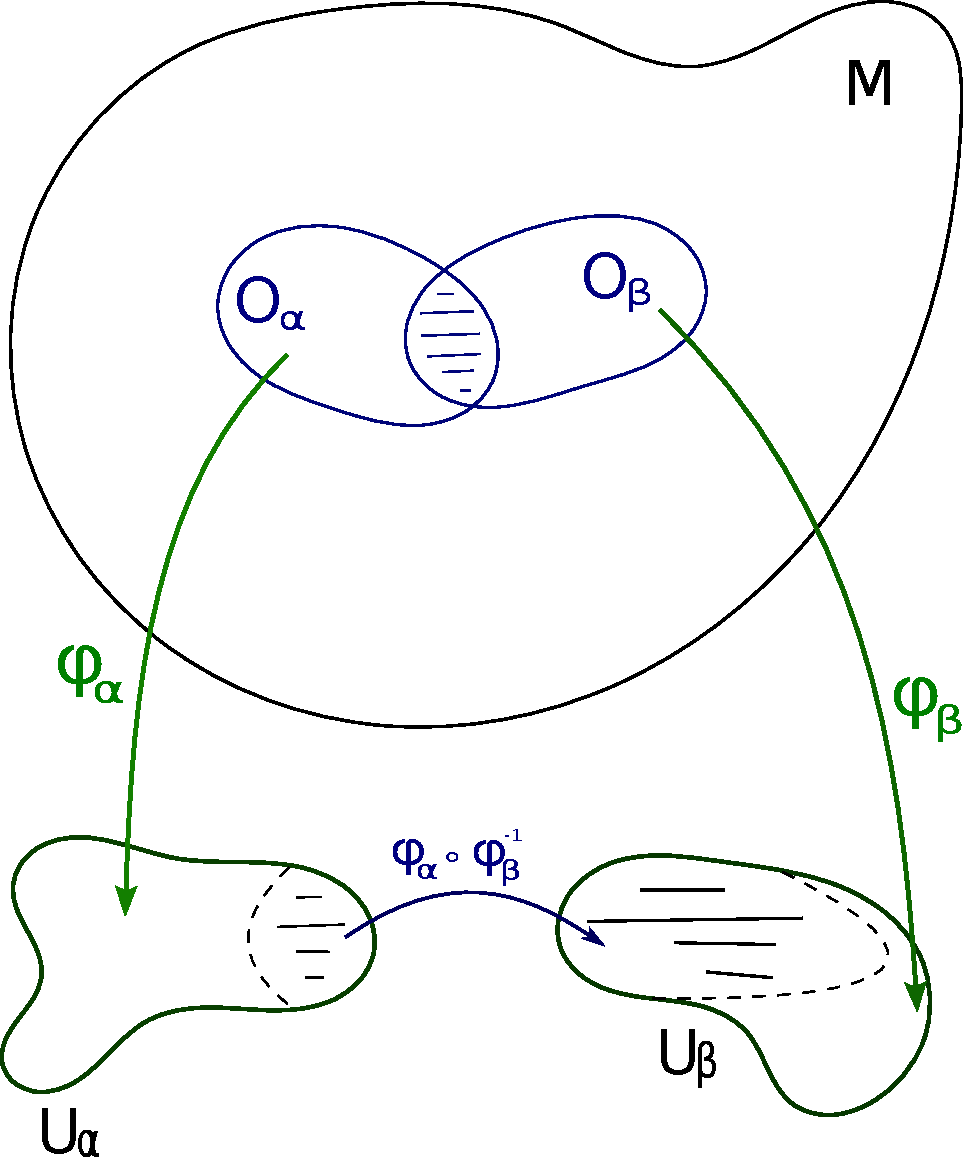
\includegraphics[width = 0.5\textwidth]{Chapter 2/Figures/TercerPostu.pdf}
            \caption{Schematic representation of the third postulate: in a differentiable manifold we can always pass from one coordinate chart to another.}
            \label{fig:TercerPostu}
        \end{figure}

        Here we must make some comments and observations:

        \begin{itemize}
            \item The maps $\phi_{\alpha}$ are usually called coordinate charts or coordinate systems, and we will later see that this is directly related to the strong equivalence principle.

            \item The collection $\{\phi_{\alpha}\}$ is called an \textit{atlas}.

            \item A point $p$ represented in a coordinate chart $\phi_{\alpha}$ is written as $\phi_{\alpha}(p) = \left(x_{\alpha}^1(p),...,x_{\alpha}^n(p)\right)$, and the components $x_{\alpha}^i$ are called the coordinates of $p$ in that chart.
        \end{itemize}
    \end{enumerate}

    We will often use the word \textit{smooth}, which refers to the differentiability of the geometrical object: we say something is smooth if it is of class $C^{\infty}$, meaning that it is infinitely differentiable. Such objects are sometimes hard to come by in practice, especially in physics, so one often works instead with objects of class $C^k$, that is, $k$ times differentiable. Let us see some examples:

    \begin{enumerate}
        \item $\mathbb{R}^n$ is itself a manifold, whose atlas consists of the single identity chart

        \begin{equation}
            \begin{split}
                \phi\;:\;\mathbb{R}^n &\longrightarrow \mathbb{R}^n\\
                (x^1,...,x^n) &\longmapsto (x^1,...,x^n).
            \end{split}
        \end{equation}

        This is a manifold of dimension $n$.

        \item $S^1$, also called the unit circle, $S^1 = \{(x,y) \in \mathbb{R}^2 \;:\; x^2 + y^2 = 1 \}$. It is a one dimensional manifold, because we only need one parameter to describe it, and at the same time it is a subset of $\mathbb{R}^2$ given by $(\cos\theta,\sin\theta)$ with $\theta \in \mathbb{R}$. Let us see how to cover this manifold.

        \begin{figure}[h]
            \centering
            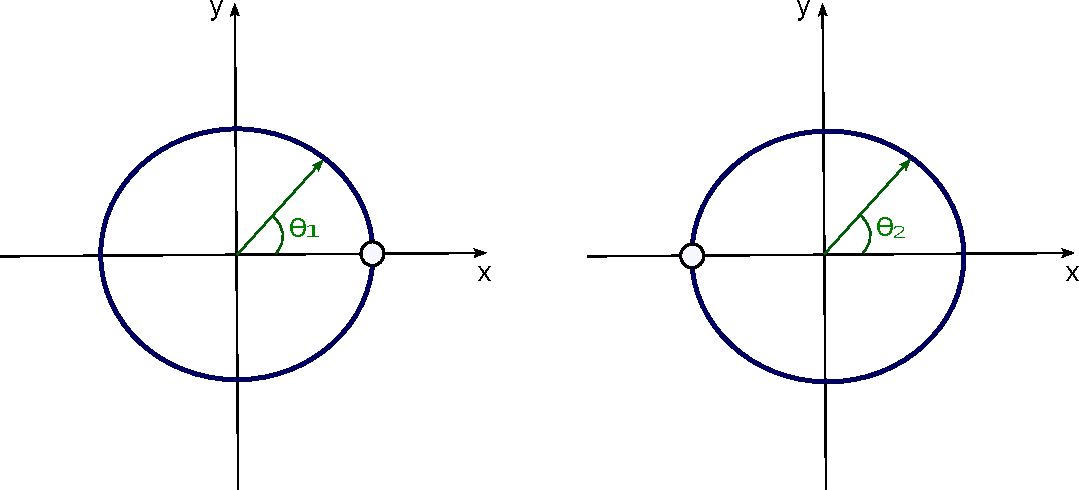
\includegraphics[width = 0.9\textwidth]{Chapter 2/Figures/CartasS1.pdf}
            \caption{On the left there is the first chart $\phi_1$, which covers almost all of the circumference except a point $p$, and on the right there is the other chart, which covers almost all of the circumference except a point $q$ diametrically opposite to $p$.}
            \label{fig:CartasS1}
        \end{figure}

        We cannot use a single closed interval, say $0 \leq \theta \leq 2\pi$, because then the map $\phi = \theta$ would fail to be bijective, since $\theta = 0$ and $\theta = 2\pi$ label the very same point of the circle. Because of this we choose two coordinate charts. Removing the point $p = (1,0)$ we define the domain $\mathcal{O}_1 = S^1 \setminus \{p\}$ and the chart

        \begin{equation}
            \begin{split}
                \phi_1\;:\;\mathcal{O}_1 &\longrightarrow (0,2\pi)\\
                (\cos\theta_1,\sin\theta_1) &\longmapsto \theta_1,
            \end{split}
        \end{equation}

        and removing instead the diametrically opposite point $q = (-1,0)$ we define $\mathcal{O}_2 = S^1 \setminus \{q\}$ together with

        \begin{equation}
            \begin{split}
                \phi_2\;:\;\mathcal{O}_2 &\longrightarrow (-\pi,\pi)\\
                (\cos\theta_2,\sin\theta_2) &\longmapsto \theta_2.
            \end{split}
        \end{equation}

        Neither chart alone covers the circle, but between them they leave nothing out, so the atlas for this manifold is

        \begin{equation}
            A = \{\phi_1,\phi_2\}.
        \end{equation}

        Now, how are $\theta_1$ and $\theta_2$ related on the region where both charts are defined? Notice first that the overlap $\mathcal{O}_1 \cap \mathcal{O}_2$ is the circle with \textit{two} points removed, so it consists of two disjoint arcs, the upper one and the lower one, and the transition function has to be given separately on each of them. From the third postulate we obtain

        \begin{equation}\label{eq:TransitionS1}
            \theta_2 = \left(\phi_2 \circ \phi_1^{-1}\right)(\theta_1) =
            \begin{cases}
                \theta_1, & 0 < \theta_1 < \pi \quad \text{(upper arc)},\\
                \theta_1 - 2\pi, & \pi < \theta_1 < 2\pi \quad \text{(lower arc)}.
            \end{cases}
        \end{equation}

        On each arc separately this is a smooth (indeed linear) function of $\theta_1$, which is exactly what the third postulate demands, and the geometrical reading of the second branch is simply that \textit{the two charts disagree by one complete turn on the lower arc}, which is the price of having cut the circle open at two different places.

        \item $S^2$, the sphere of unit radius, $S^2 = \{(x,y,z) \in \mathbb{R}^3\;:\;x^2 + y^2 + z^2 = 1\}$. Here the situation is analogous to $S^1$, because any point on the sphere has a small enough neighbourhood that maps one to one onto a disc of $\mathbb{R}^2$, see figure \ref{fig:S2toR2}.

        \begin{figure}[h]
            \centering
            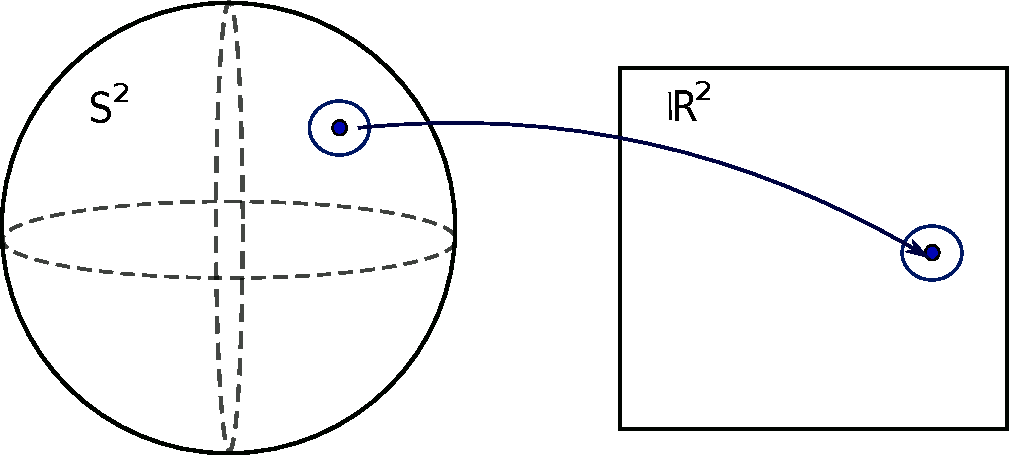
\includegraphics[width = 0.8\textwidth]{Chapter 2/Figures/S2toR2.pdf}
            \caption{Each point on the sphere has a small neighbourhood which maps onto a disc in $\mathbb{R}^2$.}
            \label{fig:S2toR2}
        \end{figure}

        This also illustrates that such a map certainly preserves neither lengths nor angles. Consider the spherical coordinates we always use in our calculus courses, taking the polar angle $\vartheta = x$ and the azimuthal angle $\varphi = y$, so that the sphere appears to be mapped onto the rectangle

        \begin{equation*}
            0 \leq x \leq \pi, \;\; 0 \leq y \leq 2\pi.
        \end{equation*}

        The map breaks down at the pole, $\vartheta = 0$. The whole pole, which is a single point of the manifold, is smeared out along the entire line $x = 0$, $0 \leq y \leq 2\pi$, see figure \ref{fig:SphereMap}, so at the pole there is no bijection and therefore no chart at all.

        \begin{figure}
            \centering
            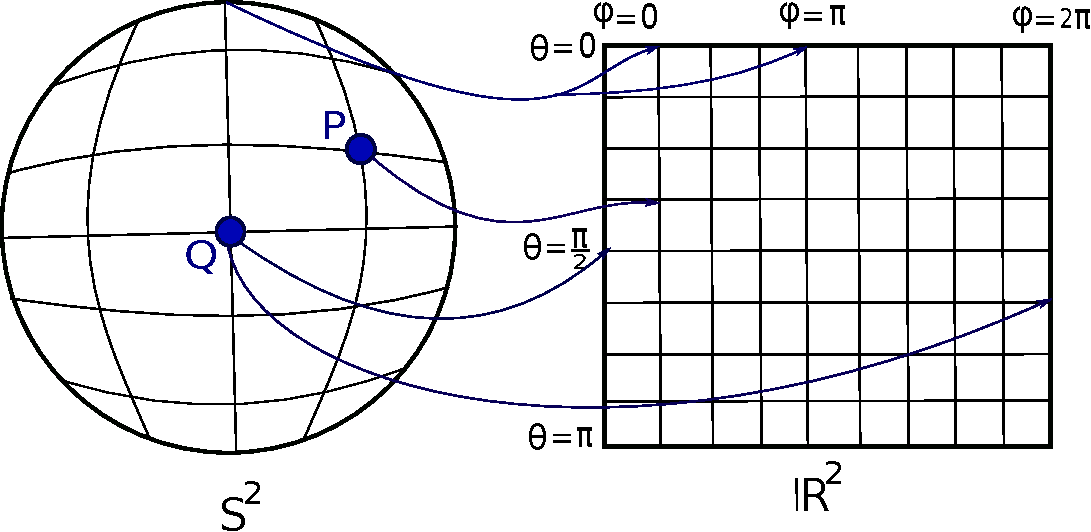
\includegraphics[width = 0.8\textwidth]{Chapter 2/Figures/SphereMap.pdf}
            \caption{Representation of the traditional map from $S^2$ to $\mathbb{R}^2$. We can see that there are multivalued points which will not allow us to cover the manifold $S^2$ with a single chart.}
            \label{fig:SphereMap}
        \end{figure}

        A second problem arises at the points whose azimuthal coordinate is $\varphi = 0$, since they are sent to both $y = 0$ and $y = 2\pi$ at once, so again the correspondence fails to be one to one.

        Both problems disappear if instead of a closed rectangle we take the open one, $0 < x < \pi$ and $0 < y < 2\pi$, and then use a second chart to cover what the first one lost, choosing for instance a chart whose own excluded line is the meridian $\varphi = \pi$, so that its azimuthal coordinate runs from $\varphi = \pi/2$ to $\varphi = 3\pi/2$.

        There is another, more elegant way to choose the charts for $S^2$, called the stereographic projection of the manifold onto $\mathbb{R}^2$.

        \begin{figure}[h]
            \centering
            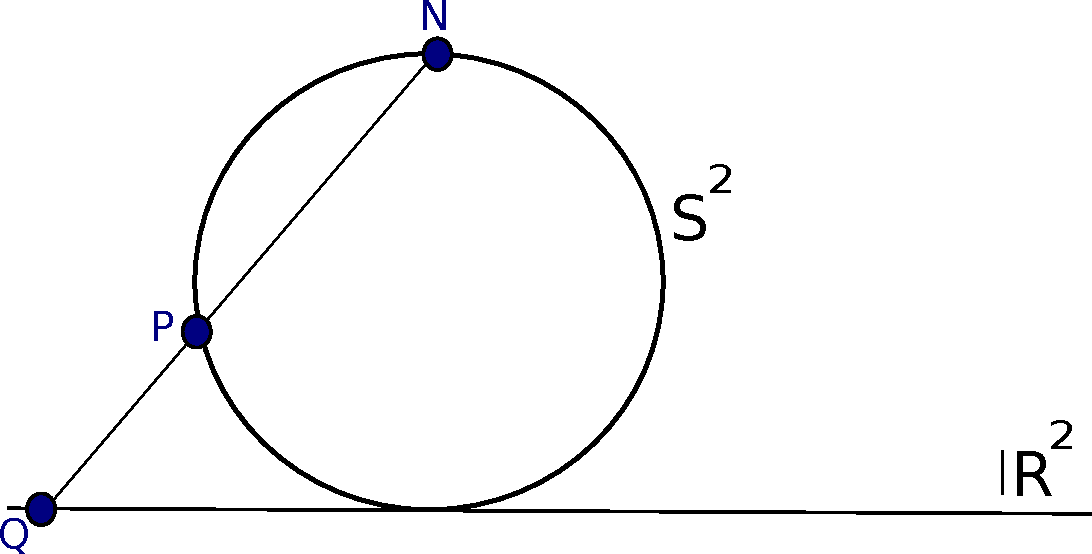
\includegraphics[width = 0.7\textwidth]{Chapter 2/Figures/Estereo.pdf}
            \caption{Graphical representation used to find the stereographic projection of $S^2$ onto $\mathbb{R}^2$.}
            \label{fig:Estereo}
        \end{figure}

        The sphere is tangent to the plane, and from the point $N$ diametrically opposite to the point of tangency we draw a straight line which cuts the sphere at $P$ and the plane $\mathbb{R}^2$ at $Q$. This defines the map: $P$ is sent to $Q$, so that the coordinates of $Q$ in $\mathbb{R}^2$ serve as the coordinates of $P$ in $S^2$. It is one to one everywhere except at $N$ itself, since as $P$ approaches $N$ the image point $Q$ runs off to infinity, and to cover $N$ we simply choose a second stereographic chart projecting from the opposite pole.
    \end{enumerate}

    \begin{myDef}
        Two atlases are compatible if their union is again an atlas. \textit{The union of all mutually compatible atlases is called the \textbf{complete atlas}}, and it is characterised by the property that it is not contained in any larger atlas.
    \end{myDef}

    \subsection{Smooth functions}

        If $\phi \;: \mathcal{O} \rightarrow U$ is a coordinate chart and $f\;: M \rightarrow \mathbb{R}$ is a function on the manifold, then the composition $f \circ \phi^{-1}$ is a map from $U \subset \mathbb{R}^n$ to $\mathbb{R}$, and this is the object we can actually differentiate, because it is an ordinary function of $n$ real variables. This is the standard manoeuvre of the whole subject: \textbf{we never differentiate on the manifold itself, we always push the problem down into $\mathbb{R}^n$ with a chart, do the calculus there, and then check that the answer did not depend on which chart we chose}.

        \begin{figure}[h]
            \centering
            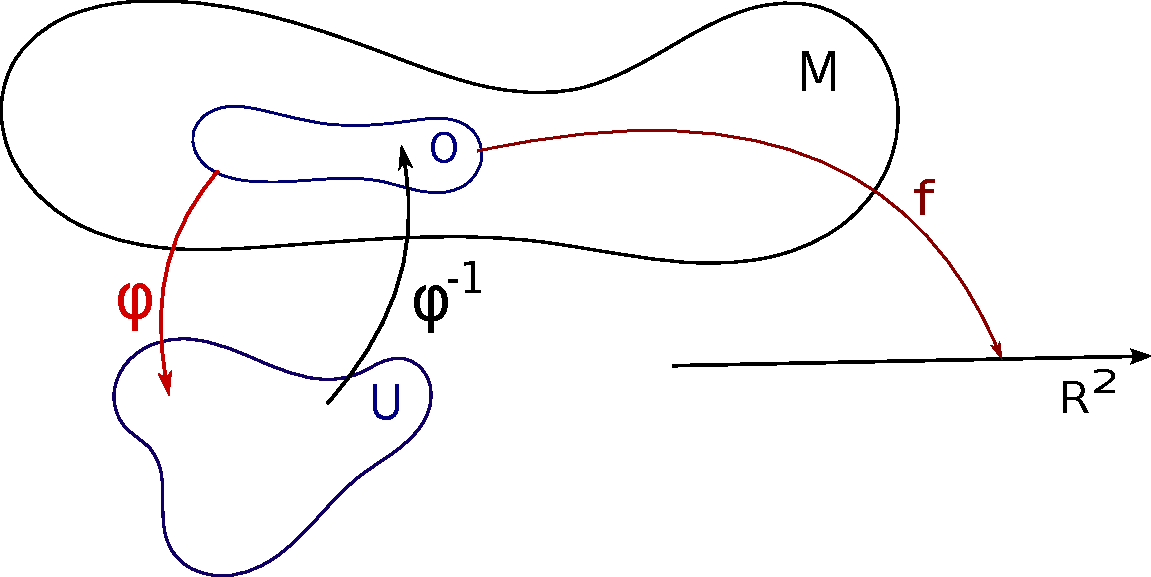
\includegraphics[width = 0.7\textwidth]{Chapter 2/Figures/SmoothFunc.pdf}
            \caption{Schematic representation of the map $f$, which takes elements of the manifold and maps them onto the real line $\mathbb{R}$.}
            \label{fig:SmoothFunc}
        \end{figure}

        \begin{myDef}
            A function

            \begin{equation}
                \begin{split}
                    f\;:\;M &\longrightarrow \mathbb{R}\\
                    p &\longmapsto f(p)
                \end{split}
            \end{equation}

            is smooth if and only if, for every coordinate chart $\phi$, the map $F \equiv f  \circ \phi^{-1}$ defined by

            \begin{equation}
                \begin{split}
                    F\;:\;U \subset \mathbb{R}^n &\longrightarrow \mathbb{R}\\
                    x &\longmapsto F(x) = f\left(\phi^{-1}(x)\right)
                \end{split}
            \end{equation}

            is a smooth function in the ordinary sense of multivariable calculus.
        \end{myDef}

        In general relativity a function $f\;:M \rightarrow \mathbb{R}$ is often called a \textit{scalar field}. The set of all such smooth functions on $M$ is denoted $C^{\infty}(M)$, and we shall need it in a moment, because tangent vectors are going to be defined as operators acting on it.

    \subsection{Curves and vectors}

        \begin{myDef}
            A smooth curve on a differentiable manifold $M$ is a smooth map

            \begin{equation}
                \begin{split}
                    \lambda\;:\;I &\longrightarrow M\\
                    t &\longmapsto \lambda(t),
                \end{split}
            \end{equation}

            where $I$ is an open interval of $\mathbb{R}$.
        \end{myDef}

        This means that $\phi_{\alpha} \circ \lambda$ is a map from $I$ into $\mathbb{R}^n$ for every coordinate chart $\phi_{\alpha}$, and this is what is represented in figure \ref{fig:Curva}.

        \begin{figure}[h]
            \centering
            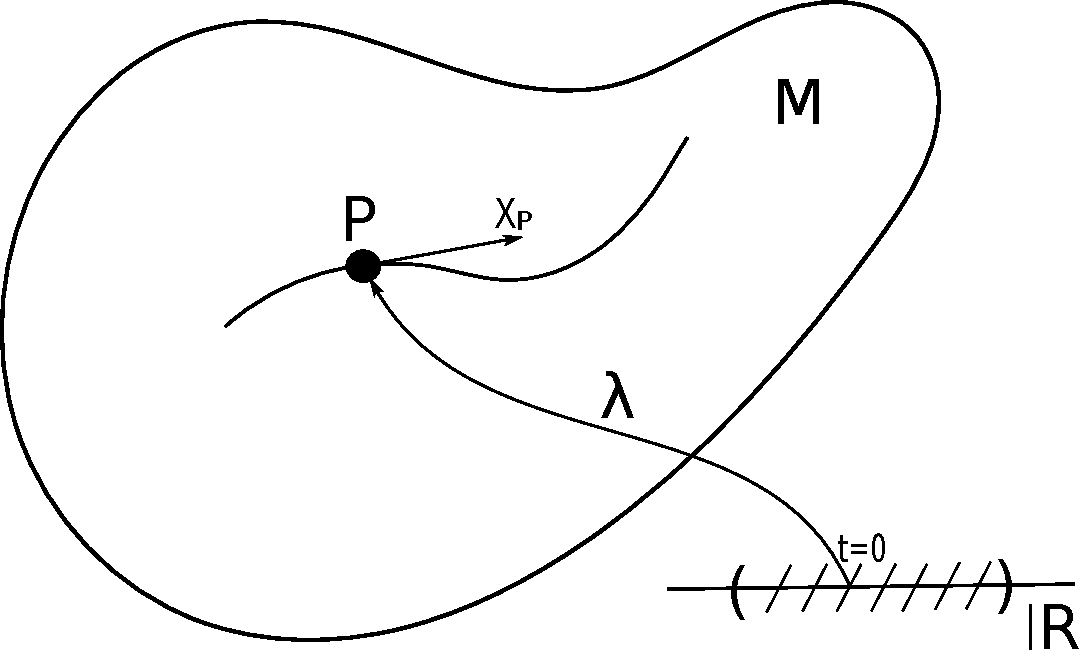
\includegraphics[width = 0.7\textwidth]{Chapter 2/Figures/Curva.pdf}
            \caption{The curve $\lambda$ maps an open interval of the reals into the manifold. On the manifold this map looks like (remember this is only a scheme) the kind of curve we are used to seeing, and at a point of that curve we can define a tangent vector $X_p$.}
            \label{fig:Curva}
        \end{figure}

        The elements of $I$ can be thought of as the parameters that parameterise the curve. Given

        \begin{equation}
            f\;:\;M \longrightarrow \mathbb{R} \;\;\text{and}\;\; \lambda\;:\;I \longrightarrow M,
        \end{equation}

        we can define the composition

        \begin{equation}
            \begin{split}
                f \circ \lambda\;:\;I &\longrightarrow \mathbb{R}\\
                t &\longmapsto f(\lambda(t)),
            \end{split}
        \end{equation}

        which is in fact a parameterised function $f(\lambda(t))$ of a single real variable, so we may perfectly well speak about its derivative with respect to the parameter $t$. To compute that derivative we must, as always, go down into a chart: writing $F = f\circ\phi^{-1}$ and $x^{\mu}(t) = x^{\mu}(\lambda(t))$ for the coordinates of the curve, the chain rule gives

        \begin{equation}\label{eq:DerivadaCurva}
            \frac{d}{dt}\left[(f\circ \lambda)(t)\right] = \frac{d}{dt}F\left(x(t)\right) = \frac{\partial F}{\partial x^{\mu}}\frac{dx^{\mu}}{dt},
        \end{equation}

        where a sum over the repeated index $\mu$ is understood. Notice that it would make no sense to write $\partial f / \partial \lambda$, since $\lambda$ takes values on the manifold and there is no notion of dividing by a point.

        \begin{myDef}
            Let $\lambda\;: I \rightarrow M$ be a smooth curve with $\lambda(0) = p$, so that the parameter value $t=0$ picks out the point $p$ on the manifold, see figure \ref{fig:Curva}. The vector tangent to $\lambda$ at $p$ is the linear map

            \begin{equation}
                \begin{split}
                    X_p\;:\;C^{\infty}(M) &\longrightarrow \mathbb{R}\\
                    f &\longmapsto X_p(f) = \left\{\frac{d}{dt}\left[f(\lambda(t))\right]\right\}_{t=0}.
                \end{split}
            \end{equation}
        \end{myDef}

        It is worth pausing on how strange this definition looks the first time one meets it. \textbf{A tangent vector is not an arrow, it is a directional derivative}, an operator that eats a function and returns the rate at which that function changes as we move along the curve. The reason for this apparently perverse choice is that arrows need an ambient space to live in, whereas directional derivatives need nothing but the manifold and its smooth functions, so this is the definition that survives when we throw the embedding space away.

        This tangent vector satisfies two really important algebraic properties.

        \begin{enumerate}
            \item The tangent vector is a linear map, so that for all $f,g \in C^{\infty}(M)$ and all $\alpha \in \mathbb{R}$,

            \begin{align}
                X_p(f+g) = X_p(f) + X_p(g),\\
                X_p(\alpha f) = \alpha X_p(f).
            \end{align}

            \item The tangent vector satisfies Leibniz's rule,

            \begin{equation}\label{eq:LeibnizXp}
                X_p(fg) = f(p) X_p(g) + g(p) X_p(f),
            \end{equation}

            where the functions multiplying the derivatives have to be evaluated at the point $p$, since $X_p(fg)$ is a number and not a function.
        \end{enumerate}

        Let us now consider a coordinate chart $\phi = (x^1,...,x^n)$ defined in a neighbourhood of $p$, and the function $F = f\circ \phi^{-1}$. Because $\phi$ is a bijection we may write

        \begin{equation}
            f\circ \lambda = f \circ \phi^{-1}\circ \phi \circ \lambda,
        \end{equation}

        or equivalently

        \begin{equation}
            f \circ \lambda = F \circ \phi \circ \lambda.
        \end{equation}

        The tangent vector, using the chain rule exactly as in equation \ref{eq:DerivadaCurva}, is then given by

        \begin{equation}\label{eq:TangentComponents}
             X_p(f) = \left\{\frac{d}{dt}\left[f(\lambda(t))\right]\right\}_{t=0} = \left(\frac{\partial F(x)}{\partial x^{\mu}}\right)_{\phi(p)} \left(\frac{dx^{\mu}(\lambda(t))}{dt}\right)_{t=0},
        \end{equation}

        which means that in general we can write every tangent vector as a linear combination of some components multiplying some basis elements, and the whole of the next page is devoted to making that statement precise.

        \begin{figure}[h]
            \centering
            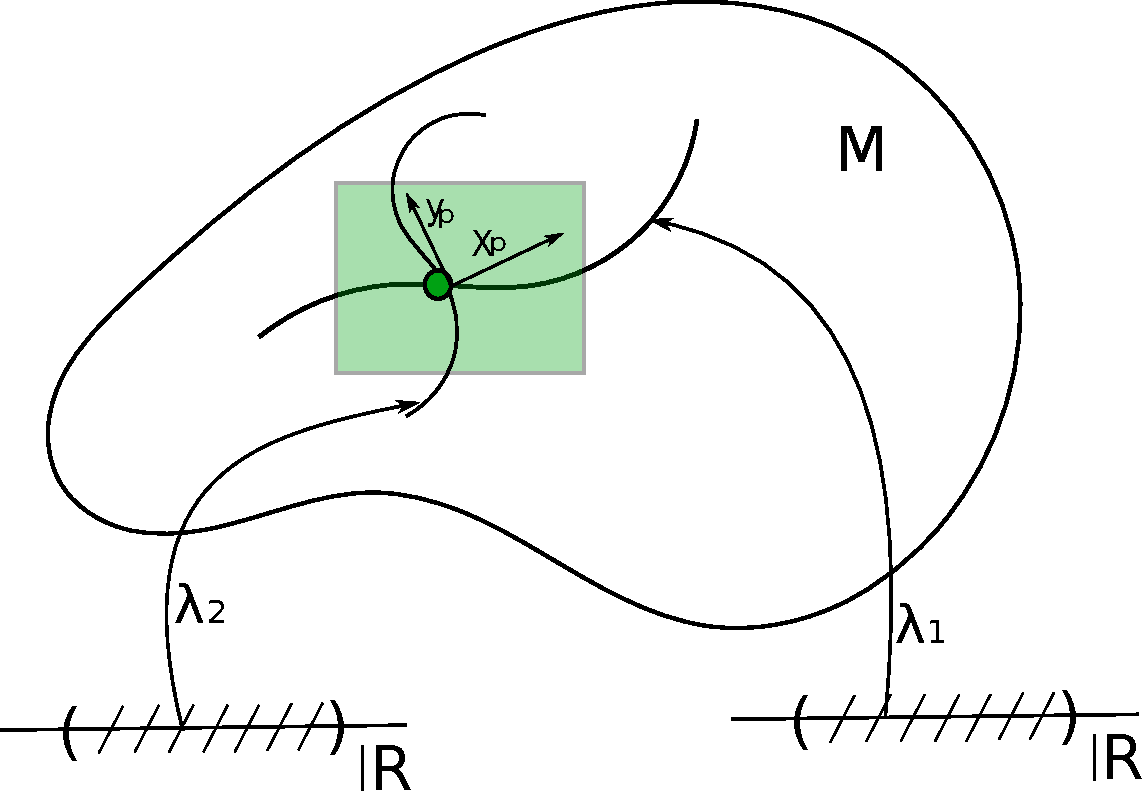
\includegraphics[width = 0.7\textwidth]{Chapter 2/Figures/Tangents.pdf}
            \caption{Two tangent vectors $X_p$ and $Y_p$, both tangent at $p$, living on two different curves $(\lambda_1,\lambda_2)$ but belonging to the same vector space $T_p(M)$.}
            \label{fig:Tangents}
        \end{figure}

        \begin{myteo}
            The set of all tangent vectors at $p$ forms an $n$-dimensional vector space, called the tangent space $T_p(M)$.
        \end{myteo}

        \textbf{\textit{Demonstration:}}\\

        Let $\lambda_1$ and $\lambda_2$ be two curves such that $\lambda_1(0) = \lambda_2(0) = p$, and let $X_p$ and $Y_p$ be their tangent vectors respectively. We must define multiplication by a constant and addition of two vectors, and to do so we exhibit a curve whose tangent is the required combination. Let $\phi = (x^1,...,x^n)$ be a coordinate chart defined in a neighbourhood of $p$ and consider the curve

        \begin{equation}
            \nu(t) = \phi^{-1}\left\{\alpha\left[\phi(\lambda_1(t)) - \phi(p)\right] + \beta\left[\phi(\lambda_2(t)) - \phi(p)\right] + \phi(p)\right\},
        \end{equation}

        which is well defined for $t$ small enough that the argument stays inside $U$, and which satisfies $\nu(0) = p$. Let $Z_p$ be the tangent vector to this curve at $p$, then

        \begin{align}
            Z_p(f) = \left(\frac{\partial F(x)}{\partial x^{\mu}}\right)_{\phi(p)}\left\{\frac{d}{dt}\left[\alpha(x^{\mu}(\lambda_1(t)) - x^{\mu}(p)) + \beta(x^{\mu}(\lambda_2(t)) - x^{\mu}(p)) + x^{\mu}(p)\right]\right\}_{t=0},\\
            Z_p(f) = \left(\frac{\partial F(x)}{\partial x^{\mu}}\right)_{\phi(p)}\left[\alpha\left(\frac{d}{dt}x^{\mu}(\lambda_1(t))\right)_{t=0} + \beta\left(\frac{d}{dt}x^{\mu}(\lambda_2(t))\right)_{t=0}\right],\\
            Z_p(f) = \alpha X_p(f) + \beta Y_p(f),\\
            Z_p(f) = (\alpha X_p + \beta Y_p)(f).
        \end{align}

        Since this holds for any smooth function $f$, we conclude that $Z_p = \alpha X_p + \beta Y_p$, and $Z_p$ is by construction tangent to the curve $\nu$ at $p$. Therefore any linear combination of tangent vectors at $p$ is again a tangent vector at $p$, and the set of tangent vectors at $p$ forms a vector space.\\

        Now we must prove that it is $n$-dimensional, and to do this we exhibit a basis. Let $1 \leq \mu \leq n$ and consider the curve $\lambda_{\mu}$ through $p$ defined by

        \begin{equation}
            \lambda_{\mu}(t) = \phi^{-1}\left(x^1(p),...,x^{\mu-1}(p),x^{\mu}(p) + t , x^{\mu + 1}(p),...,x^n(p) \right),
        \end{equation}

        that is, the curve obtained by letting the $\mu$-th coordinate run and holding all the others fixed. The tangent vector to this curve at $p$ is denoted by $\left(\frac{\partial}{\partial x^{\mu}}\right)_p$, and it acts on functions exactly as the notation suggests,

        \begin{equation}\label{eq:BasisAction}
            \left(\frac{\partial}{\partial x^{\mu}}\right)_p(f) = \left(\frac{\partial F}{\partial x^{\mu}}\right)_{\phi(p)},
        \end{equation}

        which is easy to see because we have defined $F = f \circ \phi^{-1}$ and the chart and its inverse cancel, leaving an object evaluated at $p$ rather than at $\phi(p)$.

        Let us now check that these $n$ tangent vectors are linearly independent, that is, that

        \begin{equation}
            \sum_{\mu=1}^n a_{\mu}\left(\frac{\partial}{\partial x^{\mu}}\right)_p = 0 \;\Longrightarrow\; a_1 = a_2 = ... = a_n = 0.
        \end{equation}

        The equation on the left is an equation between operators, so it means that the left hand side gives zero when applied to \textit{any} smooth function, and the cleanest way to extract the coefficients is therefore to feed it the most convenient functions we have available, namely the $n$ coordinate functions $x^{\nu}$ themselves. Applying the operator to $x^{\nu}$ and using equation \ref{eq:BasisAction} we obtain

        \begin{align*}
            0 = \sum_{\mu=1}^n a_{\mu}\left(\frac{\partial}{\partial x^{\mu}}\right)_p(x^{\nu}) = \sum_{\mu=1}^n a_{\mu}\left(\frac{\partial x^{\nu}}{\partial x^{\mu}}\right)_{\phi(p)} = \sum_{\mu=1}^n a_{\mu}\delta^{\nu}_{\;\mu} = a_{\nu},
        \end{align*}

        and since $\nu$ was arbitrary this gives

        \begin{equation}
            a_{\nu} = 0 \quad \forall \nu \in \{1,...,n\},
        \end{equation}

        which is precisely the linear independence we wanted.

        Finally, having proved that they are linearly independent, equation \ref{eq:TangentComponents} together with equation \ref{eq:BasisAction} lets us write

        \begin{equation}
            X_p(f) = \left(\frac{dx^{\mu}(\lambda(t))}{dt}\right)_{t=0}\left(\frac{\partial}{\partial x^{\mu}}\right)_p(f),
        \end{equation}

        and since this is true for every $f$ we may drop it and write the operator identity

        \begin{equation}\label{eq:VectorInBasis}
            X_p = X^{\mu}\left(\frac{\partial}{\partial x^{\mu}}\right)_p, \qquad X^{\mu} \equiv \left(\frac{dx^{\mu}(\lambda(t))}{dt}\right)_{t=0}.
        \end{equation}

        So $X_p$ can be written as a linear combination of the $n$ tangent vectors $\left(\frac{\partial}{\partial x^{\mu}}\right)_p$, which therefore span $T_p(M)$, and being also linearly independent they form a basis. This establishes that the tangent space is $n$-dimensional, the same dimension as the manifold itself.\\

        The basis $\left\{\left(\frac{\partial}{\partial x^{\mu}}\right)_p\;: \mu = 1,...,n\right\}$ depends on the coordinate chart, since we had to choose a chart $\phi$ defined in a neighbourhood of $p$ in order to build it, and choosing a different chart would give a different basis of the same space $T_p(M)$. A basis constructed in this way is called a \textit{coordinate basis}, and we will see in due course that not every basis one might want to use is of this type.\\

        We often want to represent the same object in one coordinate system or in another, so we must know how to transform both the basis vectors and the components from one representation to the other. Let $\phi = (x^1,...,x^n)$ and $\Bar{\phi}=(x^{\Bar{1}},...,x^{\Bar{n}})$ be two coordinate charts, then

        \begin{equation}
            \left(\frac{\partial}{\partial x^{\mu}}\right)_p(f) = \left(\frac{\partial}{\partial x^{\mu}}(f \circ \phi^{-1})\right)_{\phi(p)} = \left\{\frac{\partial}{\partial x^{\mu}}\left[(f\circ \Bar{\phi}^{-1})\circ(\Bar{\phi}\circ \phi^{-1})\right]\right\}_{\phi(p)},
        \end{equation}

        where we have simply inserted the identity $\Bar{\phi}^{-1}\circ\Bar{\phi}$, and writing

        \begin{equation}
            \Bar{F} = f \circ \Bar{\phi}^{-1}\;\;:\;\; \Bar{F} = \Bar{F}(\Bar{x}),
        \end{equation}

        the chain rule gives

        \begin{align*}
            \left(\frac{\partial}{\partial x^{\mu}}\right)_p(f) = \left(\frac{\partial}{\partial x^{\mu}}\left[\Bar{F}(\Bar{x}(x))\right]\right)_{\phi(p)}\\
            = \left(\frac{\partial x^{\Bar{\nu}}}{\partial x^{\mu}}\right)_{\phi(p)} \left(\frac{\partial \Bar{F}(\Bar{x})}{\partial x^{\Bar{\nu}}}\right)_{\Bar{\phi}(p)}\\
            = \left(\frac{\partial x^{\Bar{\nu}}}{\partial x^{\mu}}\right)_{\phi(p)}\left(\frac{\partial}{\partial x^{\Bar{\nu}}}\right)_p(f).
        \end{align*}

        In this way we have found the transformation rule for the \textit{basis vectors} when we pass from one coordinate system to another, which is

        \begin{equation}\label{eq:BasisTransf}
            \left(\frac{\partial}{\partial x^{\mu}}\right)_p = \left(\frac{\partial x^{\Bar{\nu}}}{\partial x^{\mu}}\right)_{\phi(p)}\left(\frac{\partial}{\partial x^{\Bar{\nu}}}\right)_p.
        \end{equation}

        The components must then transform in the opposite way, so that the vector itself, which is a geometrical object and knows nothing about our choice of chart, remains the same,

        \begin{equation}
            X_p = X^{\nu}\left(\frac{\partial}{\partial x^{\nu}}\right)_p = X^{\nu}\left(\frac{\partial x^{\Bar{\mu}}}{\partial x^{\nu}}\right)\left(\frac{\partial}{\partial x^{\Bar{\mu}}}\right)_p = X^{\Bar{\mu}}\left(\frac{\partial}{\partial x^{\Bar{\mu}}}\right)_p,
        \end{equation}

        from which we can read off the transformation law for the components,

        \begin{equation}\label{eq:CompTransf}
            X^{\Bar{\mu}} = \left(\frac{\partial x^{\Bar{\mu}}}{\partial x^{\nu}}\right)X^{\nu}.
        \end{equation}

        \textbf{Comparing equations \ref{eq:BasisTransf} and \ref{eq:CompTransf} we see that components and basis vectors transform with mutually inverse Jacobian matrices}, and this is not a coincidence, it is exactly what has to happen for the contraction $X^{\mu}(\partial/\partial x^{\mu})_p$ to come out chart independent. Objects that transform like the components in equation \ref{eq:CompTransf} are called \textit{contravariant}, and we shall meet their \textit{covariant} counterparts in the next subsection.

    \subsection{Covectors and one-forms}

        \begin{myDef}
            Let $V$ be a real vector space. The dual space $V^*$ of $V$ is the vector space of all linear maps from $V$ to the reals, that is, the space whose elements are the maps

            \begin{equation}
                \begin{split}
                    \Tilde{P}\;:\;V &\longrightarrow \mathbb{R}\\
                    X &\longmapsto \Tilde{P}(X).
                \end{split}
            \end{equation}
        \end{myDef}

        \textbf{Lemma:} if $V$ is $n$-dimensional then so is $V^*$. If $\left\{\mathbf{e}_{\mu}\;: \mu = 1,...,n\right\}$ is a basis of $V$, then $V^*$ has a basis $\{f^{\mu}\;:\mu=1,...,n\}$, called the \textit{dual basis}, defined by the condition $f^{\mu}(\mathbf{e}_{\nu}) = \delta^{\mu}_{\;\nu}$. If $X = X^{\alpha}\mathbf{e}_{\alpha}$ then the dual basis simply reads off the components,

        \begin{equation}
            f^{\alpha}(X) = f^{\alpha}\left(X^{\beta}\mathbf{e}_{\beta}\right) = X^{\beta}f^{\alpha}(\mathbf{e}_{\beta}) = X^{\beta}\delta^{\alpha}_{\;\beta} = X^{\alpha}.
        \end{equation}

        Since $V$ and $V^*$ have the same dimension they are isomorphic, so an isomorphism between them certainly exists. It is worth being careful here, though, because \textbf{that isomorphism is not canonical}: to build it we have to pick a basis of $V$ first, and a different choice of basis gives a different identification, so there is no natural way to say which covector corresponds to a given vector. In general relativity it is precisely the metric tensor that will supply the missing extra structure and let us raise and lower indices, and the fact that this requires a metric, rather than coming for free, is one of the reasons the metric occupies such a central place in the theory. The situation for the double dual is quite different.

        \begin{myteo}
            If $V$ is finite dimensional, then $(V^*)^*$ is naturally isomorphic to $V$ through the map

            \begin{equation}
                \begin{split}
                    \Psi\;:\;V &\longrightarrow (V^*)^*\\
                    X &\longmapsto \Psi(X), \quad \text{defined by}\;\; \Psi(X)(\omega) = \omega(X) \;\;\forall\;\omega \in V^*.
                \end{split}
            \end{equation}
        \end{myteo}

        Notice that no choice of basis was needed to write that map down, which is exactly what the word \textit{naturally} is doing in the statement of the theorem.

        \begin{myDef}
            The dual space of $T_p(M)$ is called the cotangent space at $p$ and is denoted by $T_p^*(M)$.
        \end{myDef}

        \begin{myDef}
            Let $f\;:M \rightarrow \mathbb{R}$ be a smooth function. The covector $(df)_p$ is defined by

            \begin{equation}
                \begin{split}
                    (df)_p\;:\;T_p(M) &\longrightarrow \mathbb{R}\\
                    X &\longmapsto (df)_p(X) = X(f),
                \end{split}
            \end{equation}

            for any $X \in T_p(M)$. It is called the differential of $f$ at $p$, or in the older physics literature the gradient of $f$ at $p$. Covectors, also called one-forms, satisfy the following properties.

            \begin{enumerate}
                \item If $\eta \in V^*$, then its components in the dual basis are recovered by acting on the basis vectors,

                \begin{equation}
                    \eta(\mathbf{e}_{\mu}) = \eta_{\nu}f^{\nu}(\mathbf{e}_{\mu}) = \eta_{\nu}\delta^{\nu}_{\;\mu} = \eta_{\mu}.
                \end{equation}

                \item If $X \in T_p(M)$, then the action of a one-form on a vector is the contraction of their components,

                \begin{equation}
                    \eta(X) = X^{\alpha}\eta_{\alpha} \in \mathbb{R}.
                \end{equation}
            \end{enumerate}
        \end{myDef}

        A one-form is a really special geometrical object, because we use it constantly in physics and yet it is usually late in our studies that we start to think about what it actually is. If vectors are pictured as directed arrows, what does a covector look like? To see this let us consider the interaction between the vector $\Vec{A} = \begin{bmatrix}
            1\\
            2
        \end{bmatrix}$ and the one-form $\Tilde{q} = \begin{bmatrix} q_1 & q_2\end{bmatrix}$, so that

        \begin{equation}\label{eq:qdeA}
            \Tilde{q}(\Vec{A}) = q_1 + 2q_2.
        \end{equation}

        If we ask which one-forms return a fixed value $c$ when fed our vector $\vec{A}$, equation \ref{eq:qdeA} tells us that the answer is the straight line $q_1 + 2q_2 = c$ in the space of components, and the family of such lines obtained by varying $c$ is a set of parallel lines whose normal has components $[1,2]^T$. Turning the picture around, this is the standard way of drawing a one-form: \textbf{while a vector is a directed arrow, a one-form is a family of parallel hyperplanes, its level surfaces, and the value $\Tilde{q}(\Vec{A})$ is the number of those surfaces that the arrow $\Vec{A}$ pierces}. A one-form with a large norm is a tightly packed stack of surfaces, and a one-form with a small norm is a loosely spaced one, which is why the picture gets the scaling right without any extra work.

        What is the most common operation that takes a scalar field and returns something orthogonal to its level surfaces? The gradient, and indeed the gradient is the archetypal example of a one-form, since it represents precisely the stack of equipotential surfaces of the field, which is the reason we denote the one-form at a point $p$ by $(df)_p$. This picture also lets us realise that in electromagnetism the electric field, written in a Coulomb gauge as $E_i = -\partial_i \varphi$, appears most naturally with its index downstairs, that is, as a one-form built as the differential of the potential, while the object we habitually draw as a field of arrows is really doing something slightly different, a point we shall be able to make completely precise once we have the metric at our disposal.

    \subsection{Tensors}

        A tensor of type $\binom{r}{s}$ at $p$ is a multilinear map

        \begin{equation}
            \begin{split}
                T\;:\;\underbrace{T_p^*(M) \times ... \times T_p^*(M)}_{r\;\text{copies}}\times \underbrace{T_p(M) \times ... \times T_p(M)}_{s\;\text{copies}} &\longrightarrow \mathbb{R}\\
                (\Tilde{q}_1,...,\Tilde{q}_r,\Vec{A}_1,...,\Vec{A}_s) &\longmapsto T(\Tilde{q}_1,...,\Tilde{q}_r,\Vec{A}_1,...,\Vec{A}_s),
            \end{split}
        \end{equation}

        which maps $r$ one-forms and $s$ vectors into the reals, the word \textit{multilinear} meaning that it is linear in each of its arguments separately when all the others are held fixed. The components of the tensor in a given basis are obtained by feeding it the basis elements themselves,

        \begin{equation}
            T^{\mu_1\;...\;\mu_r}_{\quad\;\;\nu_1\;...\;\nu_s} = T(f^{\mu_1},...,f^{\mu_r},\mathbf{e}_{\nu_1},...,\mathbf{e}_{\nu_s}),
        \end{equation}

        and it is a useful sanity check to note that a $\binom{1}{0}$ tensor is just a vector, a $\binom{0}{1}$ tensor is just a one-form, and a $\binom{0}{0}$ tensor is a scalar.

        \begin{myDef}
            If $S$ is a tensor of type $\binom{p}{q}$ and $T$ is a tensor of type $\binom{r}{s}$, then the tensor product of $S$ and $T$, denoted $S \otimes T$, is the tensor of type $\binom{p + r }{q + s}$ defined by

            \begin{equation}
                \left(S \otimes T\right)(\omega_1,...,\omega_p,\eta_1,...,\eta_r,X_1,...,X_q,Y_1,...,Y_s) = S(\omega_1,...,\omega_p,X_1,...,X_q)\,T(\eta_1,...,\eta_r,Y_1,...,Y_s).
            \end{equation}
        \end{myDef}

        \textbf{The transformation law in components.} Up to this point we have defined a tensor as a multilinear machine, which is the honest and coordinate free way of doing it, but it is not the definition the reader will meet in most physics books, where a tensor is instead introduced as \textit{a collection of numbers which transforms in a particular way under a change of coordinates}. The two definitions are completely equivalent and it is worth deriving the second from the first, because the second one is what we actually use whenever we sit down to compute. Everything follows from the way the bases transform: we already know from equation \ref{eq:BasisTransf} how the coordinate basis of $T_p(M)$ behaves, and inverting that relation gives

        \begin{equation}\label{eq:BasisTransfInv}
            \mathbf{e}_{\Bar{\nu}} = \left(\frac{\partial x^{\beta}}{\partial x^{\Bar{\nu}}}\right)\mathbf{e}_{\beta},
        \end{equation}

        while the dual basis has to transform in the opposite way, since the defining condition $f^{\mu}(\mathbf{e}_{\nu}) = \delta^{\mu}_{\;\nu}$ must remain true in every chart, and therefore

        \begin{equation}\label{eq:DualBasisTransf}
            f^{\Bar{\mu}} = \left(\frac{\partial x^{\Bar{\mu}}}{\partial x^{\alpha}}\right)f^{\alpha}.
        \end{equation}

        Now we only have to feed the barred bases into the tensor and use multilinearity to pull every Jacobian out of its slot, which gives

        \begin{equation}\label{eq:TensorTransf}
            T^{\Bar{\mu}_1...\Bar{\mu}_r}_{\quad\;\;\Bar{\nu}_1...\Bar{\nu}_s} = \frac{\partial x^{\Bar{\mu}_1}}{\partial x^{\alpha_1}}\;...\;\frac{\partial x^{\Bar{\mu}_r}}{\partial x^{\alpha_r}}\;\frac{\partial x^{\beta_1}}{\partial x^{\Bar{\nu}_1}}\;...\;\frac{\partial x^{\beta_s}}{\partial x^{\Bar{\nu}_s}}\;T^{\alpha_1...\alpha_r}_{\quad\;\;\beta_1...\beta_s},
        \end{equation}

        which is the law every physicist eventually learns by heart. The rule it encodes is simple enough to state in one sentence: \textbf{each index brings its own Jacobian, the indices upstairs carry $\partial x^{\Bar{\mu}}/\partial x^{\alpha}$ and the indices downstairs carry $\partial x^{\beta}/\partial x^{\Bar{\nu}}$}, and the whole content of the older definition of a tensor is the demand that equation \ref{eq:TensorTransf} should hold. That definition sounds circular the first time one hears it, since it seems to say that a tensor is whatever transforms like a tensor, but it is perfectly precise and it is enormously useful in practice, because it converts the question \textit{is this object geometrical?} into a mechanical check that can be carried out with nothing more than the chain rule.

        \textbf{Contraction.} There is one operation on tensors which has no analogue for ordinary numbers and which we shall use constantly from chapter 3 onwards, and it consists in setting one upper index equal to one lower index and summing over it.

        \begin{myDef}
            Let $T$ be a tensor of type $\binom{r}{s}$ with $r \geq 1$ and $s \geq 1$. The contraction of $T$ on its $i$-th contravariant and $j$-th covariant slot is the tensor of type $\binom{r-1}{s-1}$ whose components are obtained by setting those two indices equal and summing,

            \begin{equation}
                \left(C\,T\right)^{\mu_1...\mu_{r-1}}_{\qquad\nu_1...\nu_{s-1}} = T^{\mu_1...\,\alpha\,...\mu_{r-1}}_{\qquad\quad\nu_1...\,\alpha\,...\nu_{s-1}}.
            \end{equation}
        \end{myDef}

        The reason this deserves a definition of its own, rather than being dismissed as an obvious piece of index bookkeeping, is that it is genuinely surprising that the result should be a tensor at all, since we have summed over a label which only makes sense once a chart has been chosen. That it works is a small miracle of index placement, and the cleanest way to see it is to contract a $\binom{1}{1}$ tensor and watch what the Jacobians do,

        \begin{align*}
            T^{\Bar{\alpha}}_{\;\Bar{\alpha}} = {\color{red}\frac{\partial x^{\Bar{\alpha}}}{\partial x^{\mu}}\frac{\partial x^{\nu}}{\partial x^{\Bar{\alpha}}}}T^{\mu}_{\;\nu} = {\color{red}\delta^{\nu}_{\;\mu}}T^{\mu}_{\;\nu} = T^{\mu}_{\;\mu},
        \end{align*}

        where the two Jacobians marked in red have collapsed into a Kronecker delta precisely because one of them came from an upper index and the other from a lower one, so that they are inverse matrices being multiplied together. \textbf{Contraction is only legitimate between one upper and one lower index}, and an expression such as $T^{\mu\mu}$, with both indices upstairs, is not chart independent and therefore does not define anything geometrical, at least not until we have a metric available to lower one of them for us. The reader has in fact been contracting tensors for years without calling it that: the trace of a matrix, the divergence of a vector field, the scalar product written as $\omega_{\mu}X^{\mu}$ and the invariant $F^{\mu\nu}F_{\mu\nu}$ of electromagnetism are all contractions, and in chapter 3 the Ricci tensor and the Ricci scalar will be built out of the Riemann tensor by exactly this operation and nothing else.

        \textbf{Symmetric and antisymmetric parts.} Any tensor with two or more indices of the same kind can be split into a part which does not care about the order of those indices and a part which changes sign when they are swapped, and because the physically important tensors of relativity are almost always one or the other it pays to fix the notation now. We write the symmetric and antisymmetric parts with round and square brackets respectively,

        \begin{align}
            T_{(\mu\nu)} = \frac{1}{2}\left(T_{\mu\nu} + T_{\nu\mu}\right),\\
            T_{[\mu\nu]} = \frac{1}{2}\left(T_{\mu\nu} - T_{\nu\mu}\right),
        \end{align}

        and adding the two of them recovers the original tensor,

        \begin{equation}
            T_{\mu\nu} = T_{(\mu\nu)} + T_{[\mu\nu]},
        \end{equation}

        so that the splitting loses no information at all. For more than two indices the same brackets mean the average over all the permutations of the enclosed indices, with a minus sign for the odd permutations in the antisymmetric case, so that for three indices we would write $T_{[\mu\nu\rho]} = \frac{1}{3!}\left(T_{\mu\nu\rho} + T_{\nu\rho\mu} + T_{\rho\mu\nu} - T_{\nu\mu\rho} - T_{\mu\rho\nu} - T_{\rho\nu\mu}\right)$.

        Two properties make this splitting worth the trouble. The first is that \textbf{being symmetric or antisymmetric is a statement about the tensor and not about the chart}, which we can check directly by transforming a symmetric tensor and swapping the barred indices,

        \begin{align*}
            T_{\Bar{\nu}\Bar{\mu}} = \frac{\partial x^{\alpha}}{\partial x^{\Bar{\nu}}}\frac{\partial x^{\beta}}{\partial x^{\Bar{\mu}}}T_{\alpha\beta} = \frac{\partial x^{\beta}}{\partial x^{\Bar{\mu}}}\frac{\partial x^{\alpha}}{\partial x^{\Bar{\nu}}}T_{\beta\alpha} = T_{\Bar{\mu}\Bar{\nu}},
        \end{align*}

        where we used the symmetry $T_{\alpha\beta} = T_{\beta\alpha}$ and then simply renamed the two dummy indices, so a tensor which is symmetric in one coordinate system is symmetric in all of them, and the same argument with one extra minus sign works for antisymmetry. The second property is an identity we shall use again and again without comment, namely that \textbf{the full contraction of a symmetric tensor with an antisymmetric one always vanishes},

        \begin{equation}\label{eq:SymAntisym}
            S^{\mu\nu}A_{\mu\nu} = 0 \qquad \text{whenever} \;\; S^{\mu\nu} = S^{\nu\mu} \;\; \text{and} \;\; A_{\mu\nu} = -A_{\nu\mu},
        \end{equation}

        which follows in one line by using the symmetry of $S$, then the antisymmetry of $A$, and then relabelling the dummies, since this produces $S^{\mu\nu}A_{\mu\nu} = -S^{\mu\nu}A_{\mu\nu}$ and a quantity equal to minus itself can only be zero.

        Finally it is worth counting, because the counting explains a good deal of physics. In $n$ dimensions a symmetric two index tensor has $n(n+1)/2$ independent components and an antisymmetric one has $n(n-1)/2$, so in the four dimensions of space-time we get ten and six respectively. Those two numbers should look familiar: the metric $g_{\mu\nu}$ is symmetric and has exactly ten independent components, which is why Einstein's field equations are ten equations and not sixteen, while the Faraday tensor $F_{\mu\nu}$ is antisymmetric and has exactly six, which is nothing other than the three components of the electric field plus the three of the magnetic field.

    \subsection{Tensor fields}

        \begin{myDef}
            A vector field is a map $X$ which assigns to every point $p \in M$ a vector $X_p \in T_p(M)$. Acting on a smooth function it produces another function,

            \begin{equation}
                \begin{split}
                    X(f)\;:\;M &\longrightarrow \mathbb{R}\\
                    p &\longmapsto X_p(f).
                \end{split}
            \end{equation}
        \end{myDef}

        These vector fields tell us how a physical quantity may change from one point of the manifold to another. Usually we picture a vector field as a field of arrows, but that picture belongs to the manifold $\mathbb{R}^n$, and this last definition is far more general, so those abstract arrows are better interpreted as rates of change of our physical quantities. The field is smooth if $X(f)$ is a smooth function for every smooth $f$.

        \begin{myDef}
            A covector field, or one-form field, is a map $\omega$ which assigns to every point $p \in M$ a covector $\omega_p \in T_p^*(M)$, so that acting on a vector field it produces a function,

            \begin{equation}
                \begin{split}
                    \omega(\Vec{X})\;:\;M &\longrightarrow \mathbb{R}\\
                    p &\longmapsto \omega_p\left(\Vec{X}_p\right).
                \end{split}
            \end{equation}
        \end{myDef}

        This is analogous to the vector field, but in this case there is no analogue of a space of arrows, and the right mental picture is instead a foliation of the manifold by the level surfaces we described above. In both cases the smoothness of the field depends on the smoothness of its components and of the functions $f$ on which it acts.

        \begin{myDef}
            A $\binom{r}{s}$ tensor field is a map $T$ which assigns to every point $p \in M$ a $\binom{r}{s}$ tensor $T_p$ at $p$,

            \begin{equation}
                \begin{split}
                    T(\eta_1,...,\eta_r,\Vec{X}_1,...,\Vec{X}_s)\;:\;M &\longrightarrow \mathbb{R}\\
                    p &\longmapsto T_p\left((\eta_1)_p ,...,(\eta_r)_p,(\Vec{X}_1)_p,...,(\Vec{X}_s)_p\right).
                \end{split}
            \end{equation}
        \end{myDef}

        Tensor fields can be thought of as the generalisation of vector and covector fields, and this is the heart of many physical theories, not only general and special relativity: they appear in solid state physics, in particle physics and even in crystal optics. They are so important because, as we will see later, with a tensor we can define the notion of distance between events \footnote{this is also related to a topology on the manifold $M$} and we can also define physical quantities that do not depend on the coordinate chart, quantities such as the Maxwell stress tensor, which tells us how much electromagnetic energy density is stored in our system, the Faraday electromagnetic tensor, which tells us how the electric and magnetic fields are related and encodes the conservation laws of a dynamical system, or the pressure tensor, which tells us about the pressure in every direction of a fluid, even in a magnetohydrodynamical one.\\

        Tensors were the heart of twentieth century physics, but there are now further geometrical objects, such as spinors, which behave in a sense like fractional rank tensors, or the twistors of Penrose, which contain both tensors and spinors.

    \subsection{Commutator}

        Let us analyse two vector fields $\Vec{X}$ and $\Vec{Y}$ acting on a smooth function $f$. Since $\Vec{Y}(f)$ is again a smooth function, we may feed it to $\Vec{X}$, and it is natural to ask whether the composition $\Vec{X}\left(\Vec{Y}(f)\right)$ is itself a vector field. To answer this we must check whether the new operator satisfies linearity and the Leibniz rule. Linearity is immediate, so let us test Leibniz by applying the composition to a product of functions,

        \begin{align*}
            \Vec{X}\left(\Vec{Y}(fg)\right) &= \Vec{X}\left( f\Vec{Y}(g) + g \Vec{Y}(f)\right)\\
            &= f \Vec{X}\left(\Vec{Y}(g)\right) + g\Vec{X}\left(\Vec{Y}(f)\right) + \Vec{X}(f)\Vec{Y}(g) + \Vec{X}(g)\Vec{Y}(f).
        \end{align*}

        The first two terms are exactly what the Leibniz rule would demand, but the last two are extra, so \textbf{the composition $\Vec{X}\circ\Vec{Y}$ is not a vector field}, essentially because applying two derivatives in a row produces second derivatives and a genuine derivation is only allowed first ones. The remedy is to notice that the two offending terms are completely symmetric under the exchange $\Vec{X}\leftrightarrow\Vec{Y}$, since repeating the computation with the fields swapped gives

        \begin{align*}
            \Vec{Y}\left(\Vec{X}(fg)\right) = f \Vec{Y}\left(\Vec{X}(g)\right) + g\Vec{Y}\left(\Vec{X}(f)\right) + \Vec{Y}(f)\Vec{X}(g) + \Vec{Y}(g)\Vec{X}(f),
        \end{align*}

        so that if we subtract one from the other the unwanted terms cancel exactly and we are left with an operator that does obey Leibniz. This motivates defining a new map $\Vec{Z}$ by

        \begin{equation}
            \Vec{Z}(f) = \Vec{X}\left(\Vec{Y}(f)\right) - \Vec{Y}\left(\Vec{X}(f)\right),
        \end{equation}

        which, by the argument we have just given, is a genuine vector field.

        \begin{myDef}
            The commutator of two vector fields $\Vec{X}$ and $\Vec{Y}$ is the vector field defined by

            \begin{equation}
                \left[\Vec{X},\Vec{Y}\right](f) = \Vec{X}\left(\Vec{Y}(f)\right) - \Vec{Y}\left(\Vec{X}(f)\right)\;\; \forall f \in C^{\infty}(M).
            \end{equation}
        \end{myDef}

        We can expand the definition of the commutator to see how it operates in a given coordinate chart $\phi = (x^1,...,x^n)$,

        \begin{align*}
            \left[\Vec{X},\Vec{Y}\right](f) &= \Vec{X}\left(Y^{\alpha}\frac{\partial F}{\partial x^{\alpha}}\right) - \Vec{Y}\left(X^{\beta}\frac{\partial F}{\partial x^{\beta}}\right)\\
            &= X^{\beta}\frac{\partial}{\partial x^{\beta}}\left(Y^{\alpha}\frac{\partial F}{\partial x^{\alpha}}\right) - Y^{\alpha}\frac{\partial}{\partial x^{\alpha}}\left(X^{\beta}\frac{\partial F}{\partial x^{\beta}} \right)\\
            &= X^{\beta}\frac{\partial Y^{\alpha}}{\partial x^{\beta}}\frac{\partial F}{\partial x^{\alpha}} + {\color{red}X^{\beta}Y^{\alpha}\frac{\partial^2 F}{\partial x^{\beta}\partial x^{\alpha}}} - Y^{\alpha}\frac{\partial X^{\beta}}{\partial x^{\alpha}}\frac{\partial F}{\partial x^{\beta}} - {\color{red}Y^{\alpha}X^{\beta}\frac{\partial^2 F}{\partial x^{\alpha}\partial x^{\beta}}},
        \end{align*}

        where the two second derivative terms marked in red cancel one another because the mixed partial derivatives of a smooth function commute, which is exactly the cancellation we anticipated above. Relabelling the dummy index in the first term so that both surviving terms carry the same derivative $\partial F/\partial x^{\beta}$, we obtain

        \begin{equation}
            \left[\Vec{X},\Vec{Y}\right](f) = \left(X^{\alpha}\frac{\partial Y^{\beta}}{\partial x^{\alpha}} - Y^{\alpha}\frac{\partial X^{\beta}}{\partial x^{\alpha}}\right)\frac{\partial F}{\partial x^{\beta}},
        \end{equation}

        so that, comparing with the expansion of a vector field in the coordinate basis,

        \begin{equation}
            \left[\Vec{X},\Vec{Y}\right](f) = \left[\Vec{X},\Vec{Y}\right]^{\beta}\left( \frac{\partial}{\partial x^{\beta}}\right)_p(f),
        \end{equation}

        we can finally read off the components of the commutator,

        \begin{equation}\label{eq:CommutatorComponents}
            \left[\Vec{X},\Vec{Y}\right]^{\beta} = X^{\alpha}\frac{\partial Y^{\beta}}{\partial x^{\alpha}} - Y^{\alpha}\frac{\partial X^{\beta}}{\partial x^{\alpha}}.
        \end{equation}

        The commutator satisfies four important relations:

        \begin{enumerate}
            \item $\left[\Vec{X},\Vec{Y}\right] = - \left[\Vec{Y},\Vec{X}\right]$; the commutator is antisymmetric.

            \item $\left[\Vec{X},\Vec{Y} + \Vec{Z}\right] = \left[\Vec{X},\Vec{Y}\right] + \left[\Vec{X},\Vec{Z}\right]$; the commutator is linear in each argument.

            \item $\left[\Vec{X},f\Vec{Y}\right] = f \left[\Vec{X},\Vec{Y}\right] + \Vec{X}(f)\Vec{Y}$; this is how the commutator behaves under multiplication by a smooth function $f$, and note that it is \textit{not} simply linear over functions, the extra term being the reason the commutator is a derivation rather than a tensor.

            \item $\left[\Vec{X},\left[\Vec{Y},\Vec{Z}\right]\right] + \left[\Vec{Y},\left[\Vec{Z},\Vec{X}\right]\right] + \left[\Vec{Z},\left[\Vec{X},\Vec{Y}\right]\right] = 0$; the Jacobi identity.
        \end{enumerate}

        We will see later that this commutator carries a great deal of physical information, because the Riemann tensor, which tells us about the geometry of the system, can be written in terms of commutators, which makes its independence of any coordinate chart manifest. The second promise we made, that the commutator would tell us whether a given basis is a coordinate basis or not, we can keep immediately.

        \begin{myteo}
            Let $\{\mathbf{e}_1,...,\mathbf{e}_n\}$ be $n$ linearly independent smooth vector fields defined on some region of a manifold $M$. There exists a coordinate chart $\phi = (x^1,...,x^n)$ on that region such that $\mathbf{e}_{\mu} = \partial/\partial x^{\mu}$ for every $\mu$, which is to say the basis is a coordinate basis, if and only if all of the commutators vanish,

            \begin{equation}\label{eq:CoordBasisCriterion}
                \left[\mathbf{e}_{\mu},\mathbf{e}_{\nu}\right] = 0 \qquad \forall\; \mu,\nu.
            \end{equation}
        \end{myteo}

        \textbf{\textit{Demonstration of the easy direction:}}\\

        Suppose the basis is a coordinate basis, so that $\mathbf{e}_{\mu} = \partial/\partial x^{\mu}$ for some chart. Then applying the commutator to any smooth function and going down into that chart, as we have done throughout this section, gives

        \begin{align*}
            \left[\frac{\partial}{\partial x^{\mu}},\frac{\partial}{\partial x^{\nu}}\right](f) = \frac{\partial^2 F}{\partial x^{\mu}\partial x^{\nu}} - \frac{\partial^2 F}{\partial x^{\nu}\partial x^{\mu}} = 0,
        \end{align*}

        which vanishes because $F$ is smooth and the mixed partial derivatives of a smooth function of several real variables do not depend on the order in which they are taken. The converse, that vanishing commutators guarantee that coordinates exist, is genuinely harder and is a consequence of the Frobenius theorem, whose proof we shall not reproduce here and which the interested reader can find in \citet{wald1984} or in \citet{nakahara2003}.

        The geometrical content of equation \ref{eq:CoordBasisCriterion} is much more intuitive than the algebra suggests, and it is worth carrying the picture around because exactly the same picture returns when we build the Riemann tensor in chapter 3. Take two vector fields $\Vec{X}$ and $\Vec{Y}$, start at a point $p$, travel a parameter distance $\epsilon$ along the integral curve of $\Vec{X}$ and then a parameter distance $\epsilon$ along the integral curve of $\Vec{Y}$, and note where you land. Now do the same two journeys in the opposite order. \textbf{In general you do not arrive at the same point, and the gap between the two endpoints is $\epsilon^2\left[\Vec{X},\Vec{Y}\right]$ to lowest order}, so the commutator is precisely the failure of the little parallelogram to close \citep{mtw1973}. A coordinate system is nothing but a grid, and a grid closes by construction, since going three steps east and then two steps north must land you where going two steps north and then three steps east does, and that is the whole reason coordinate bases are exactly the bases with vanishing commutators.

        It is worth finishing with an example which usually surprises people, because it shows that a basis every physicist has used since their first year is not a coordinate basis at all. Take the plane in polar coordinates $(r,\theta)$ and the orthonormal basis we all draw on such a diagram, which is

        \begin{equation}
            \hat{\mathbf{e}}_r = \frac{\partial}{\partial r},\qquad \hat{\mathbf{e}}_{\theta} = \frac{1}{r}\frac{\partial}{\partial \theta},
        \end{equation}

        where the factor $1/r$ is there precisely so that $\hat{\mathbf{e}}_{\theta}$ has unit length rather than length $r$. Computing the commutator with equation \ref{eq:CommutatorComponents}, or simply acting on a function and being careful with the product rule, we find

        \begin{align*}
            \left[\hat{\mathbf{e}}_r,\hat{\mathbf{e}}_{\theta}\right](f) = \frac{\partial}{\partial r}\left(\frac{1}{r}\frac{\partial f}{\partial \theta}\right) - \frac{1}{r}\frac{\partial}{\partial \theta}\left(\frac{\partial f}{\partial r}\right) = -\frac{1}{r^2}\frac{\partial f}{\partial \theta} = -\frac{1}{r}\hat{\mathbf{e}}_{\theta}(f),
        \end{align*}

        so that

        \begin{equation}
            \left[\hat{\mathbf{e}}_r,\hat{\mathbf{e}}_{\theta}\right] = -\frac{1}{r}\hat{\mathbf{e}}_{\theta} \neq 0.
        \end{equation}

        \textbf{The orthonormal polar basis is therefore not a coordinate basis}, and there is no coordinate system anywhere whose partial derivatives are $\hat{\mathbf{e}}_r$ and $\hat{\mathbf{e}}_{\theta}$, which is the honest reason behind all those extra terms that appear when one writes the divergence or the Laplacian in polar coordinates and which students usually memorise without ever being told where they come from. Bases of this kind, with non vanishing commutators, are called \textit{anholonomic} or non coordinate bases, and far from being pathological they are extremely useful in relativity, since an observer carrying a set of orthonormal rods and a clock is carrying exactly such a basis and not a coordinate one.

    \subsection{Integral curves}

        In ordinary language the terms curve and vector field are used as though they described separate things, but if we look carefully they are not separate at all. If we go back to our elementary calculus courses we remember that in $\mathbb{R}^3$ a curve is given by a vector whose components are parameterised functions, and that is exactly what we have been developing here: a curve is a map from an interval $I$, parameterised by $t$, into the manifold, which in the case of $\mathbb{R}^3$ is represented by the familiar $\lambda(t) = [X(t),Y(t),Z(t)]^T$.\\

        It is time to formalise all of this, and the mental picture to keep in mind is the velocity field of a fluid, which (and not only in special relativity) is usually written as a vector field $\Vec{U}(\Vec{X}) \in \mathbb{R}^3$. The trajectory followed by a particle carried along by that velocity field is fixed by an initial position $\Vec{X}_0$ through

        \begin{equation}\label{eq:curvaintegral}
            \frac{d \Vec{X}}{dt} = \Vec{U}\left(\Vec{X}(t)\right)\;;\;\Vec{X}(0) = \Vec{X}_0,
        \end{equation}

        and the solution of equation \ref{eq:curvaintegral} is what we call the \textit{integral curve of $\Vec{U}$ through $\Vec{X}_0$}.

        \begin{myDef}
            Let $\Vec{X}$ be a vector field on a manifold $M$ and let $p \in M$. An integral curve of $\Vec{X}$ through $p$ is a curve passing through $p$ whose tangent vector at every point coincides with the value of $\Vec{X}$ at that point.
        \end{myDef}

        Let $\lambda$ be an integral curve of $\Vec{X}$ with $\lambda(0) = p$, and choose a coordinate chart $\phi = (x^1,...,x^n)$. Writing the condition that the tangent of the curve equals the field at every point, component by component, gives the system of ordinary differential equations

        \begin{equation}\label{eq:IntegralCurveODE}
            \frac{d}{dt}\left[x^{\alpha}(\lambda(t))\right] = X^{\alpha}\left(\lambda(t)\right),
        \end{equation}

        subject to the initial condition

        \begin{equation}
            x^{\alpha}(\lambda(0)) = x^{\alpha}(p).
        \end{equation}

        Since the components $X^{\alpha}$ are smooth functions of the coordinates, the standard existence and uniqueness theorem for ordinary differential equations guarantees that through every point $p$ there passes exactly one integral curve, at least for a short enough interval of the parameter $t$. \textbf{The initial condition is what selects one curve out of the whole family}, and if we drop it we are left with the family itself, which is precisely the setting in which one speaks of the flow of the vector field, of autonomous and non autonomous dynamical systems, and eventually of chaos.

    \subsection{A worked example: the two sphere}

        Everything we have built so far has been abstract on purpose, since the whole point of the construction is that it never refers to an ambient space, but abstraction is much easier to trust once one has seen it produce familiar answers in a case where the answers are already known. In this subsection we are going to take the unit sphere $S^2$, which we already met as an example of a manifold, and compute absolutely everything explicitly: the coordinate basis, a curve and its tangent vector, a non coordinate basis, the commutators, a change of chart and an integral curve. The reader who works through this once will find the rest of the book considerably less intimidating.

        \textbf{The chart and the coordinate basis.} We work on the region covered by the usual spherical chart, $\phi = (\vartheta,\varphi)$ with $0 < \vartheta < \pi$ and $0 < \varphi < 2\pi$, which as we discussed above misses one meridian and both poles, so strictly speaking we are working on one patch of an atlas which needs at least two. The coordinate basis of the tangent space at each point of the patch is

        \begin{equation}
            \left\{\left(\frac{\partial}{\partial \vartheta}\right)_p,\;\left(\frac{\partial}{\partial \varphi}\right)_p\right\},
        \end{equation}

        and since there are two of them the tangent space $T_p(S^2)$ is two dimensional, exactly as the general theorem promised, which is already worth noticing: \textbf{the tangent space to the sphere is a plane of two dimensions and not of three}, even though we habitually draw the sphere sitting inside $\mathbb{R}^3$, because the manifold itself is two dimensional and the third dimension in the drawing is our own addition and nothing the sphere knows about.

        \textbf{A curve and its tangent vector.} Consider the circle of constant latitude at $\vartheta = \vartheta_0$, described by the curve

        \begin{equation}
            \lambda(t) = \phi^{-1}\left(\vartheta_0, \varphi_0 + t\right),
        \end{equation}

        whose coordinates are $\vartheta(t) = \vartheta_0$ and $\varphi(t) = \varphi_0 + t$. Using equation \ref{eq:VectorInBasis} its tangent vector has components $X^{\vartheta} = d\vartheta/dt = 0$ and $X^{\varphi} = d\varphi/dt = 1$, so that

        \begin{equation}
            X_p = \left(\frac{\partial}{\partial \varphi}\right)_p,
        \end{equation}

        which says that the vector field $\partial/\partial\varphi$ is precisely the field whose integral curves are the circles of latitude, travelled once per $2\pi$ of parameter. This is the generator of rotations about the polar axis and we will meet it again in a moment.

        \textbf{A basis which is not a coordinate basis.} Physicists almost never use the coordinate basis on a sphere, because $\partial/\partial\varphi$ does not have unit length, its length being $\sin\vartheta$, which shrinks to nothing as we approach the poles. What we use instead is the orthonormal basis

        \begin{equation}
            \hat{\mathbf{e}}_{\vartheta} = \frac{\partial}{\partial \vartheta},\qquad \hat{\mathbf{e}}_{\varphi} = \frac{1}{\sin\vartheta}\frac{\partial}{\partial \varphi},
        \end{equation}

        and by the criterion of equation \ref{eq:CoordBasisCriterion} we can now ask whether this is a coordinate basis, which amounts to computing one commutator,

        \begin{align*}
            \left[\hat{\mathbf{e}}_{\vartheta},\hat{\mathbf{e}}_{\varphi}\right](f) &= \frac{\partial}{\partial \vartheta}\left(\frac{1}{\sin\vartheta}\frac{\partial f}{\partial \varphi}\right) - \frac{1}{\sin\vartheta}\frac{\partial}{\partial \varphi}\left(\frac{\partial f}{\partial \vartheta}\right)\\
            &= -\frac{\cos\vartheta}{\sin^2\vartheta}\frac{\partial f}{\partial \varphi} + {\color{red}\frac{1}{\sin\vartheta}\frac{\partial^2 f}{\partial \vartheta \partial \varphi}} - {\color{red}\frac{1}{\sin\vartheta}\frac{\partial^2 f}{\partial \varphi \partial \vartheta}}\\
            &= -\frac{\cos\vartheta}{\sin\vartheta}\left(\frac{1}{\sin\vartheta}\frac{\partial f}{\partial \varphi}\right) = -\cot\vartheta\;\hat{\mathbf{e}}_{\varphi}(f),
        \end{align*}

        where the second derivative terms marked in red cancel as always, and therefore

        \begin{equation}
            \left[\hat{\mathbf{e}}_{\vartheta},\hat{\mathbf{e}}_{\varphi}\right] = -\cot\vartheta\;\hat{\mathbf{e}}_{\varphi} \neq 0.
        \end{equation}

        So the orthonormal basis on the sphere, exactly like the orthonormal polar basis on the plane, is anholonomic, and no coordinate system exists whose partial derivatives are $\hat{\mathbf{e}}_{\vartheta}$ and $\hat{\mathbf{e}}_{\varphi}$.

        \textbf{The rotation generators and an old friend.} The sphere has three obvious symmetries, the rotations about the three Cartesian axes, and each of them is generated by a vector field on $S^2$. Written in our chart they are

        \begin{align}
            \Vec{X}_{(z)} &= \frac{\partial}{\partial \varphi},\\
            \Vec{X}_{(x)} &= -\sin\varphi\frac{\partial}{\partial \vartheta} - \cos\varphi\cot\vartheta\frac{\partial}{\partial \varphi},\\
            \Vec{X}_{(y)} &= \cos\varphi\frac{\partial}{\partial \vartheta} - \sin\varphi\cot\vartheta\frac{\partial}{\partial \varphi},
        \end{align}

        and computing their commutators with equation \ref{eq:CommutatorComponents}, which is a slightly tedious but completely mechanical exercise that the reader should do at least once, gives

        \begin{align}
            \left[\Vec{X}_{(x)},\Vec{X}_{(y)}\right] = -\Vec{X}_{(z)},\\
            \left[\Vec{X}_{(y)},\Vec{X}_{(z)}\right] = -\Vec{X}_{(x)},\\
            \left[\Vec{X}_{(z)},\Vec{X}_{(x)}\right] = -\Vec{X}_{(y)}.
        \end{align}

        This should stop the reader in their tracks, because it is the angular momentum algebra of quantum mechanics arriving unannounced in the middle of a geometry calculation. If we define the operators $\hat{L}_i = -i\hbar\Vec{X}_{(i)}$, which is exactly how the angular momentum operators are built in any quantum mechanics course \citep{sakurai2011}, then the three relations above become

        \begin{equation}
            \left[\hat{L}_x,\hat{L}_y\right] = i\hbar\hat{L}_z,
        \end{equation}

        together with its cyclic partners, and \textbf{the commutation relations that a physics student first meets as an algebraic curiosity about operators turn out to be a purely geometrical statement about how rotations fail to commute on the surface of a sphere}. The overall sign is a matter of convention, since flipping the sign of all three fields flips the sign of the structure constants, but the content does not depend on that choice.

        \textbf{A change of chart.} Let us now check equation \ref{eq:BasisTransf} on a concrete change of coordinates, using the stereographic projection we described earlier. Projecting from the north pole onto the plane tangent at the south pole gives the chart $(u,v)$ with

        \begin{equation}
            u = 2\cot\left(\frac{\vartheta}{2}\right)\cos\varphi,\qquad v = 2\cot\left(\frac{\vartheta}{2}\right)\sin\varphi,
        \end{equation}

        so that the distance from the origin in the plane is $R = \sqrt{u^2+v^2} = 2\cot(\vartheta/2)$, which correctly runs off to infinity as we approach the north pole at $\vartheta = 0$ and vanishes at the south pole at $\vartheta = \pi$. Applying the transformation law for basis vectors, which simply means computing the Jacobian of this change and contracting, we obtain

        \begin{align}
            \frac{\partial}{\partial \varphi} &= \frac{\partial u}{\partial \varphi}\frac{\partial}{\partial u} + \frac{\partial v}{\partial \varphi}\frac{\partial}{\partial v} = -v\frac{\partial}{\partial u} + u\frac{\partial}{\partial v},\\
            \frac{\partial}{\partial \vartheta} &= \frac{\partial u}{\partial \vartheta}\frac{\partial}{\partial u} + \frac{\partial v}{\partial \vartheta}\frac{\partial}{\partial v} = -\frac{4 + R^2}{4R}\left(u\frac{\partial}{\partial u} + v\frac{\partial}{\partial v}\right).
        \end{align}

        The first of these is worth reading twice, because $-v\,\partial_u + u\,\partial_v$ is exactly the generator of rotations in the plane that we all wrote down in first year mechanics, and it has appeared here automatically: the field which rotates the sphere about its polar axis is, seen through the stereographic chart, the field which rotates the plane about its origin. The second one is a pure radial field, which is the projection of the meridians, and both expressions are perfectly regular everywhere except at the origin of the plane and at infinity, which are the two points where this single chart is bound to fail.

        \textbf{An integral curve, and a warning.} Finally let us solve equation \ref{eq:IntegralCurveODE} for the field $\Vec{X}_{(z)} = \partial/\partial\varphi$, whose components are $X^{\vartheta}=0$ and $X^{\varphi}=1$, so that the system reads

        \begin{equation}
            \frac{d\vartheta}{dt} = 0,\qquad \frac{d\varphi}{dt} = 1,
        \end{equation}

        with the immediate solution $\vartheta(t) = \vartheta_0$ and $\varphi(t) = \varphi_0 + t$, which is the circle of latitude we started from, closing the loop of this example. There is, however, one last thing the sphere has to teach us, and it is topological rather than geometrical: the field $\partial/\partial\varphi$ vanishes at both poles, since there is no preferred direction of rotation once you are standing exactly on the axis, and this is not a defect of our particular choice. \textbf{Every smooth vector field on $S^2$ must vanish somewhere}, a result proved by Brouwer in 1912 and known affectionately as the hairy ball theorem, because it says you cannot comb a hairy sphere flat without leaving at least one crown. The plane and the torus suffer from no such obstruction, so this is a genuine statement about the shape of the sphere and not about our charts, and it is a first hint that manifolds carry global information that no amount of local calculus will ever reveal.

    \subsection{Why the partial derivative is not enough}

        We are about to start differentiating tensor fields, and before we do it is essential to understand why the obvious candidate fails, because the failure is what forces the whole apparatus of the next section and of the next chapter into existence. The obvious candidate is simply to take the components of a vector field and differentiate them one by one, forming the array $\partial V^{\nu}/\partial x^{\mu}$, which certainly looks like the components of a $\binom{1}{1}$ tensor since it carries one index upstairs and one downstairs. Let us test it against equation \ref{eq:TensorTransf} and see whether it really transforms as it should.

        Starting from the transformation law for the components of a vector, equation \ref{eq:CompTransf}, and differentiating with the chain rule,

        \begin{align*}
            \frac{\partial V^{\Bar{\mu}}}{\partial x^{\Bar{\alpha}}} = \frac{\partial x^{\beta}}{\partial x^{\Bar{\alpha}}}\frac{\partial}{\partial x^{\beta}}\left(\frac{\partial x^{\Bar{\mu}}}{\partial x^{\nu}}V^{\nu}\right) = \underbrace{\frac{\partial x^{\beta}}{\partial x^{\Bar{\alpha}}}\frac{\partial x^{\Bar{\mu}}}{\partial x^{\nu}}\frac{\partial V^{\nu}}{\partial x^{\beta}}}_{\text{what a tensor would do}} + \underbrace{\frac{\partial x^{\beta}}{\partial x^{\Bar{\alpha}}}\frac{\partial^2 x^{\Bar{\mu}}}{\partial x^{\beta}\partial x^{\nu}}V^{\nu}}_{\text{the unwanted term}},
        \end{align*}

        we see that the first term is exactly the transformation law a $\binom{1}{1}$ tensor is supposed to obey, one Jacobian upstairs and one downstairs, but that there is a second term which has no business being there, and \textbf{because of it the partial derivative of the components of a vector field is not a tensor}. The offending term is built from the second derivatives of the coordinate change, so it vanishes if and only if those second derivatives vanish, which happens exactly when the change of coordinates is affine, that is, linear plus a constant shift.

        That observation explains a great deal about why relativity is taught the way it is. \textbf{Lorentz transformations are linear}, so in special relativity the second derivatives are identically zero, the unwanted term never appears, and a physicist can differentiate the components of a four vector with $\partial_{\mu}$ all day long and still obtain perfectly good tensors. General relativity allows arbitrary smooth changes of coordinates, which are certainly not linear, so the same manoeuvre stops working immediately, and this single fact is the reason the next chapter has to spend so much effort building a new derivative from scratch.

        There are two honest ways out of the difficulty and we shall use both. The first is to add extra structure to the manifold, an object called a \textit{connection}, whose own transformation law contains an inhomogeneous piece designed precisely to cancel the unwanted term above, producing the \textit{covariant derivative} $\nabla_{\mu}$ that we shall construct in chapter 3 and which is the derivative appearing in the geodesic equation and in the Einstein field equations. The second is to give up on differentiating in a single direction and instead use a second vector field to carry the comparison for us, dragging the tensor along the flow of that field and comparing it with itself, which produces the \textit{Lie derivative} and which needs no extra structure whatsoever beyond the manifold itself. That second route is the subject of the section which follows.

        It is worth closing with a small consolation, because the situation is not quite as bad as it looks. If we take a one-form instead of a vector and run the same computation, the unwanted term turns out to be

        \begin{equation}
            \frac{\partial^2 x^{\alpha}}{\partial x^{\Bar{\nu}}\partial x^{\Bar{\mu}}}\omega_{\alpha},
        \end{equation}

        which is manifestly symmetric under the exchange of $\Bar{\mu}$ and $\Bar{\nu}$, since mixed partial derivatives commute, so if we antisymmetrise the two indices using the brackets we introduced above then the whole offending term disappears and

        \begin{equation}
            \partial_{[\mu}\omega_{\nu]} \;\;\text{is a tensor},
        \end{equation}

        even though $\partial_{\mu}\omega_{\nu}$ on its own is not. This is not an accident, it is the first appearance of the \textit{exterior derivative}, the one derivative in differential geometry that needs no connection at all, and it is the reason the electromagnetic field tensor $F_{\mu\nu} = \partial_{\mu}A_{\nu} - \partial_{\nu}A_{\mu}$ is a perfectly good tensor in curved space-time despite being written entirely with ordinary partial derivatives.

\section{The Lie derivative}

    There is a truly important concept in general relativity and differential geometry, the derivative, but there is no single derivative, there are many kinds and all of them have their own meaning and applications: the ordinary derivative, the partial derivative, the gradient, the divergence, the curl, the Jacobian, the covariant derivative, the fractional derivative. Here we are going to develop one special derivative that allows us to pull or push elements from one manifold to another, and to find the notion of a derivative along a curve together with the relation between manifolds which are in general different. These are the pull back and push forward operations, and with them we can develop the \textit{Lie derivative}, a kind of primitive and primordial derivative of which the scalar, partial and even the covariant derivative are particular cases.

    \subsection{Pull back and push forward}

        Let $M$ and $N$ be two different manifolds, let $f$ be a smooth function mapping from $N$ to $\mathbb{R}$, and let $\phi$ be a bijection mapping from $M$ to $N$. There then exists an inverse map $\phi^{-1}: N \rightarrow M$ such that $\phi \circ\phi^{-1} = I_N$, where $I_N$ is the identity function on the manifold $N$, and $\phi^{-1}\circ \phi = I_M$, where $I_M$ is the identity function on the manifold $M$.\\
